% Options for packages loaded elsewhere
\PassOptionsToPackage{unicode}{hyperref}
\PassOptionsToPackage{hyphens}{url}
%
\documentclass[
]{article}
\usepackage{lmodern}
\usepackage{amssymb,amsmath}
\usepackage{ifxetex,ifluatex}
\ifnum 0\ifxetex 1\fi\ifluatex 1\fi=0 % if pdftex
  \usepackage[T1]{fontenc}
  \usepackage[utf8]{inputenc}
  \usepackage{textcomp} % provide euro and other symbols
\else % if luatex or xetex
  \usepackage{unicode-math}
  \defaultfontfeatures{Scale=MatchLowercase}
  \defaultfontfeatures[\rmfamily]{Ligatures=TeX,Scale=1}
\fi
% Use upquote if available, for straight quotes in verbatim environments
\IfFileExists{upquote.sty}{\usepackage{upquote}}{}
\IfFileExists{microtype.sty}{% use microtype if available
  \usepackage[]{microtype}
  \UseMicrotypeSet[protrusion]{basicmath} % disable protrusion for tt fonts
}{}
\usepackage{xcolor}
\IfFileExists{xurl.sty}{\usepackage{xurl}}{} % add URL line breaks if available
\IfFileExists{bookmark.sty}{\usepackage{bookmark}}{\usepackage{hyperref}}
\hypersetup{
  pdftitle={Ecology Counts!},
  pdfauthor={Odalys Barrientos, Brianna Cirillo, Veronia Marquez},
  hidelinks,
  pdfcreator={LaTeX via pandoc}}
\urlstyle{same} % disable monospaced font for URLs
\usepackage[margin=1in]{geometry}
\usepackage{graphicx,grffile}
\makeatletter
\def\maxwidth{\ifdim\Gin@nat@width>\linewidth\linewidth\else\Gin@nat@width\fi}
\def\maxheight{\ifdim\Gin@nat@height>\textheight\textheight\else\Gin@nat@height\fi}
\makeatother
% Scale images if necessary, so that they will not overflow the page
% margins by default, and it is still possible to overwrite the defaults
% using explicit options in \includegraphics[width, height, ...]{}
\setkeys{Gin}{width=\maxwidth,height=\maxheight,keepaspectratio}
% Set default figure placement to htbp
\makeatletter
\def\fps@figure{htbp}
\makeatother
\setlength{\emergencystretch}{3em} % prevent overfull lines
\providecommand{\tightlist}{%
  \setlength{\itemsep}{0pt}\setlength{\parskip}{0pt}}
\setcounter{secnumdepth}{-\maxdimen} % remove section numbering

\title{Ecology Counts!}
\author{Odalys Barrientos, Brianna Cirillo, Veronia Marquez}
\date{}

\begin{document}
\maketitle

\hypertarget{statistical-methodology}{%
\section{Statistical Methodology}\label{statistical-methodology}}

In this analysis, contingency tables were used to asses how many journal
entries came from each of the independent variables used. A contingency
table, which can also be called a cross tabulation, is a table that
shows the frequency distribution of each of the variables. Data cleaning
was performed, thus removing any data where the independent variable
being looked at was not applicable. Therefore, we separated the data by
continent, country, region, state, and ecosystem. We looked at each of
these tables to determine if the number of journal entries in each
category, of these variables, were equal or close in frequency.

In order to better understand the distribution of the number of journal
entries in each category, pie charts and bar graphs were made. This gave
a visual representation of the distribution of journal entries in each
independent variable. Therefore allowing for a visual analysis based on
graphs and tables made.

To further analyze these categories, chi square tests were used to
determine whether or not the observed amount of journal entries for each
of the independent variables were equal. The Pearson's chi-squared test
is used to determine whether there is a statistically significant
difference between the expected frequencies and the observed frequencies
in one or more categories of a contingency table. An assumption of the
test is that observations are mutually exclusive and independent.
Therefore, data cleaning was done to ensure this condition was met. But
the data was not randomly sampled, which goes against one of the
assumptions. Thus, the p-values obtained do not have any relevance or
any real meaning in relation to the data.

Being that the data consists of predominantly categorical variables,
some additional data was added. Square mileage of continent, country,
region, and state were researched, in order to better estimate the
expected number of journal entries in each category.This allowed for chi
square tests to be run with expected frequencies, that match the square
mileage of each of the independent variables. This allowed for more
accurate expected frequencies of journal entries from each independent
variable. Data cleaning was done to remove rows that did not contain
applicable data for each independent variable. The assumption of random
sampling is still violated, therefore the p-values obtained could not be
used to draw conclusions.

\hypertarget{results}{%
\section{Results}\label{results}}

\hypertarget{a.-continent}{%
\subsection{a. Continent}\label{a.-continent}}

The continent category demonstrated if any or the amount of published
articles completed their study in a particular continent. This allowed
us to see which continent were more or less commonly seen for ecology
work. The following contingency table counts the number of times a
continent was represented in the data set.
\textless\textless\textless\textless\textless\textless\textless{}
Updated upstream

\begin{figure}
    \centering
    \includegraphics[width=0.50\textwidth]{ContinentCTable.pdf}
    \label{fig:Contingency Table}
\end{figure}

From the table above notice the number of published articles is higher
in North America in comparison to the other continents.

If there is an assumption that the probability of each continent being
represented in a journal entry is the same, then there should be the
same number of counts for each continent. Below, is a XChi-Square test
that shows if this statement is true or not.

\begin{figure}
    \centering
    \includegraphics[width=0.50\textwidth]{ContinentChiSquare1.pdf}
    \label{fig:Continent XChi-Square}
\end{figure}

From the Pearson residuals notice that North America has the most
positive residual thus, the observed frequency exceeds the expected
frequency. Additionally, Australia has the most negative residual thus,
the observed frequency does not meet the expected frequency. Through
visual representation, figure \emph{\#} clarifies this idea. The pie
chart on the left shows what the pie chart should look like if every
continent had an equal chance of being represented in a published
article. While the pie chart on the right is what the pie chart looks
like when using the counts from the data set.

\begin{figure}
    \centering
    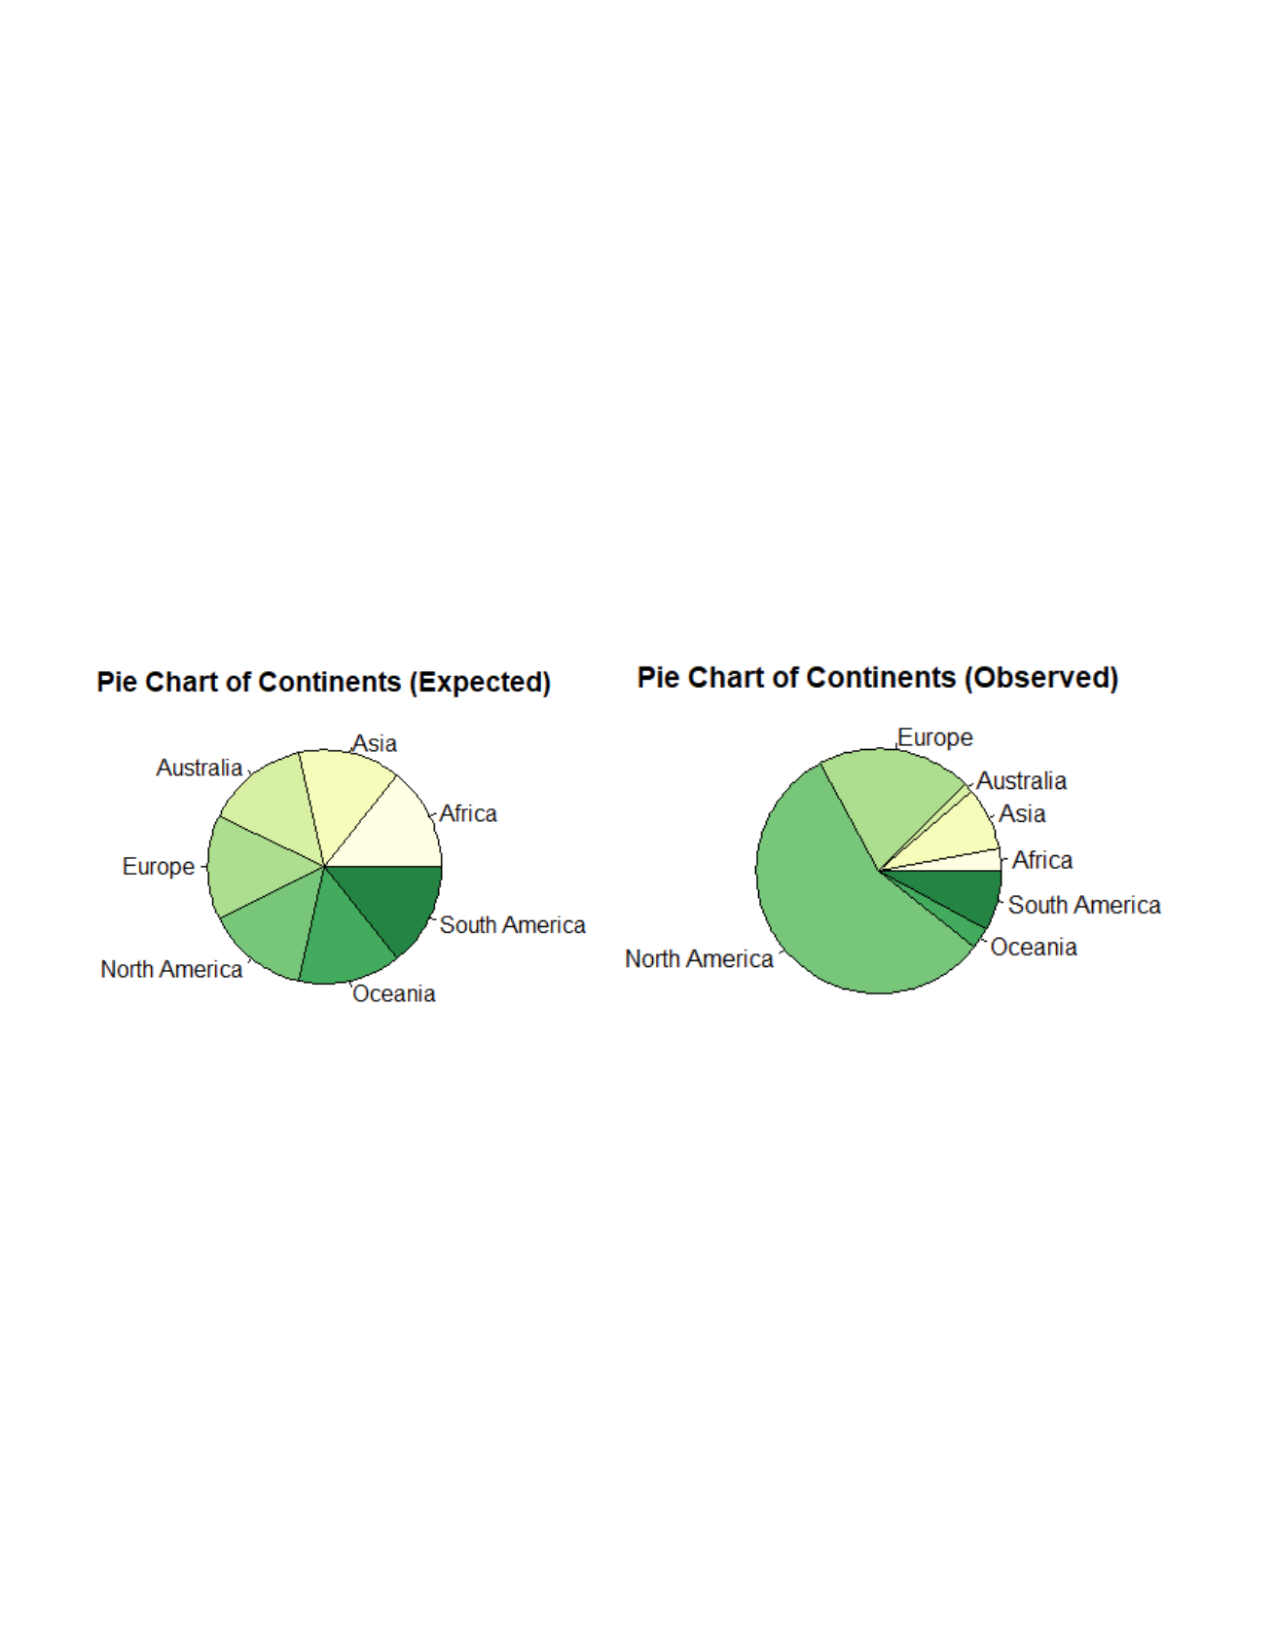
\includegraphics[width=0.50\textwidth]{ContinentPieChart.pdf}
    \label{fig:Continent Pie Chart}
\end{figure}

If the continents had a equal chance of being represented in these
published articles these pie charts would look similar. Unfortunately,
this is not the case and it is obvious that North America takes up the
majority of the pie chart.

If there is an assumption that the probability of each continent being
represented in a journal entry is the same as each continent's square
mileage. Then the continent with larger square mileage would have more
published articles than those continent with a smaller square mileage.
Below, is a XChi-Square test that shows if this statement is true or
not.

\begin{figure}
    \centering
    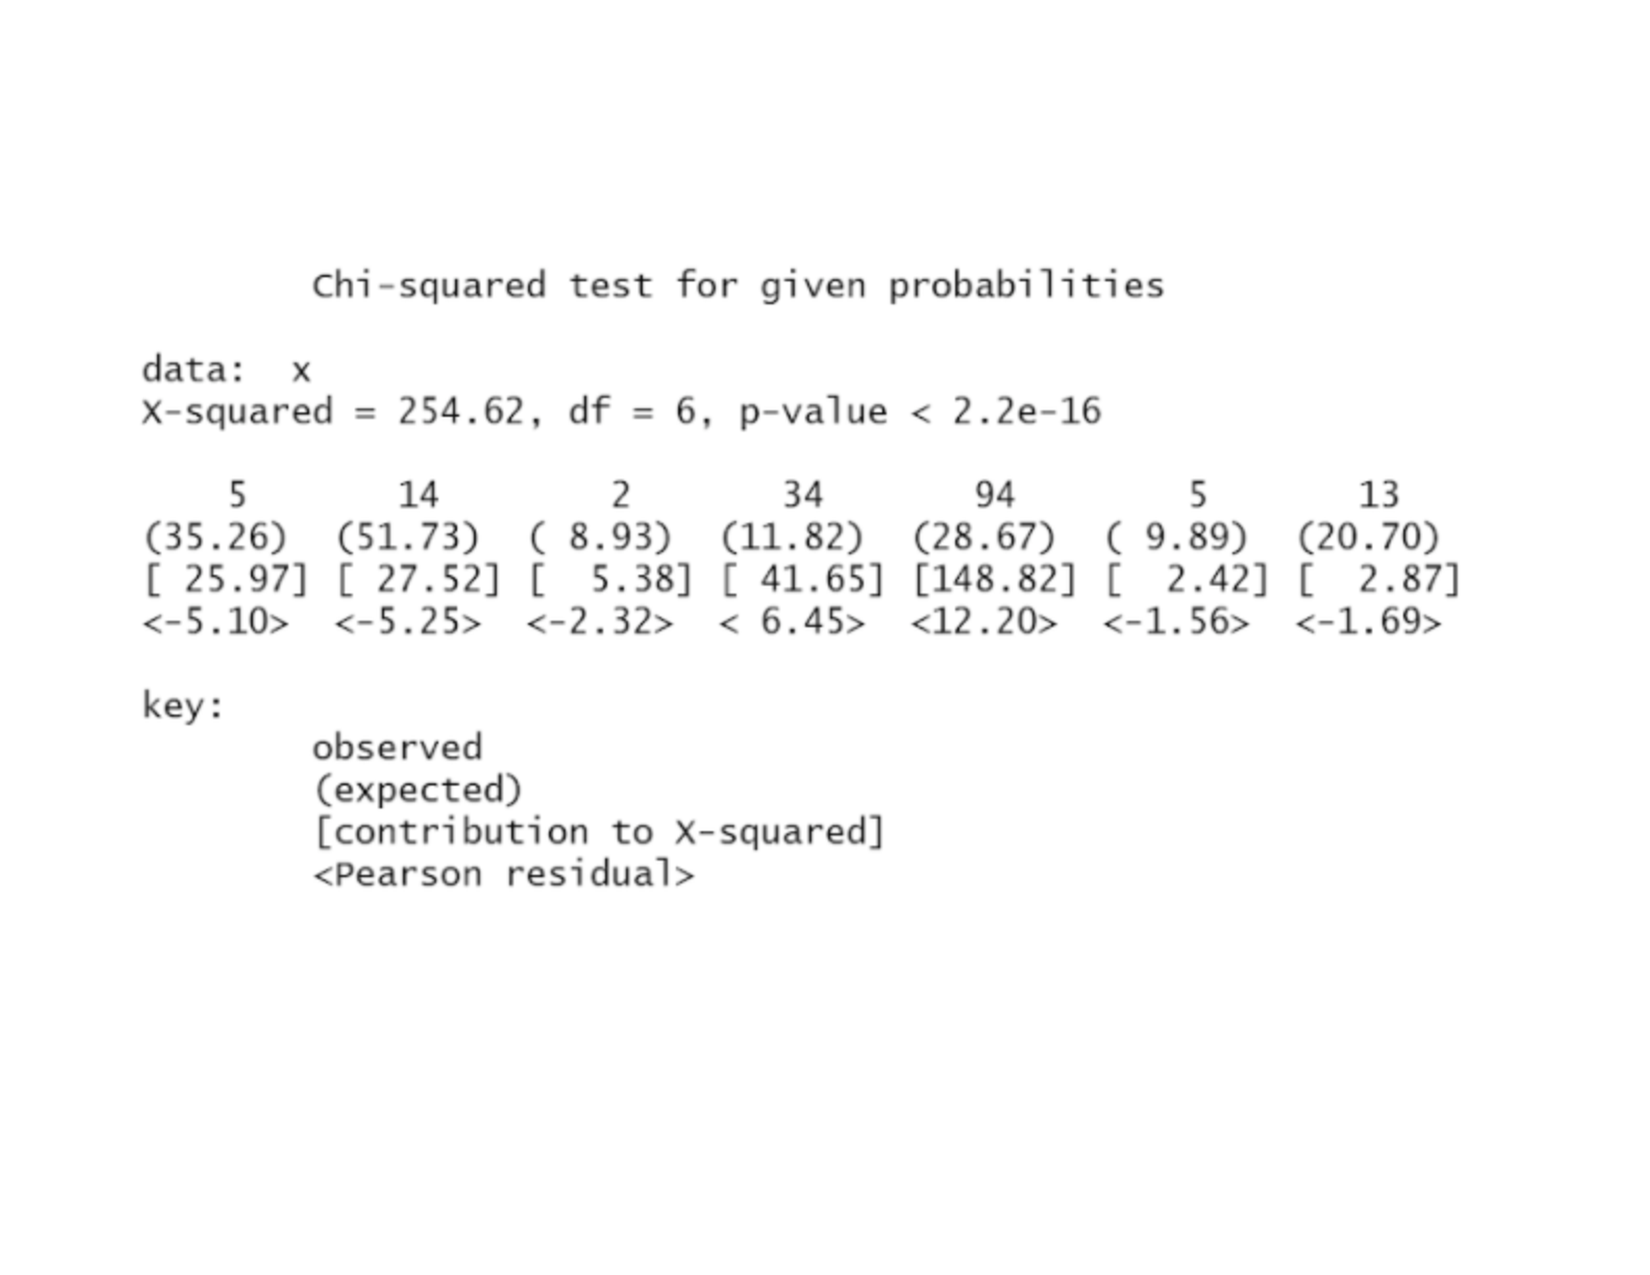
\includegraphics[width=0.50\textwidth]{ContinentChiSquare2.pdf}
    \label{fig:Continent XChi-Square}
\end{figure}

Looking into the Pearson residuals notice that North America has the
most positive residual thus showing that the observed frequency exceeds
the expected frequency. Through visual representation, figure \emph{\#}
clarifies this idea. The bar graph on the left is the number of journals
one expects to see given each continent's square mileage. The bar graph
on the right is what was observed using the counts from the data set.

\textbackslash begin\{figure\} \centering =======

\begin{figure}
    \centering
    \includegraphics[width=0.50\textwidth]{ContinentCTable.pdf}
    \label{fig:Contingency Table}
\end{figure}

From the table above notice the number of published articles is higher
in North America in comparison to the other continents.

If there is an assumption that the probability of each continent being
represented in a journal entry is the same, then there should be the
same number of counts for each continent. Below, is a XChi-Square test
that shows if this statement is true or not.

\begin{figure}
    \centering
    \includegraphics[width=0.50\textwidth]{ContinentChiSquare1.pdf}
    \label{fig:Continent XChi-Square}
\end{figure}

From the Pearson residuals notice that North America has the most
positive residual thus, the observed frequency exceeds the expected
frequency. Additionally, Australia has the most negative residual thus,
the observed frequency does not meet the expected frequency. Through
visual representation, figure \emph{\#} clarifies this idea. The pie
chart on the left shows what the pie chart should look like if every
continent had an equal chance of being represented in a published
article. While the pie chart on the right is what the pie chart looks
like when using the counts from the data set.

\begin{figure}
    \centering
    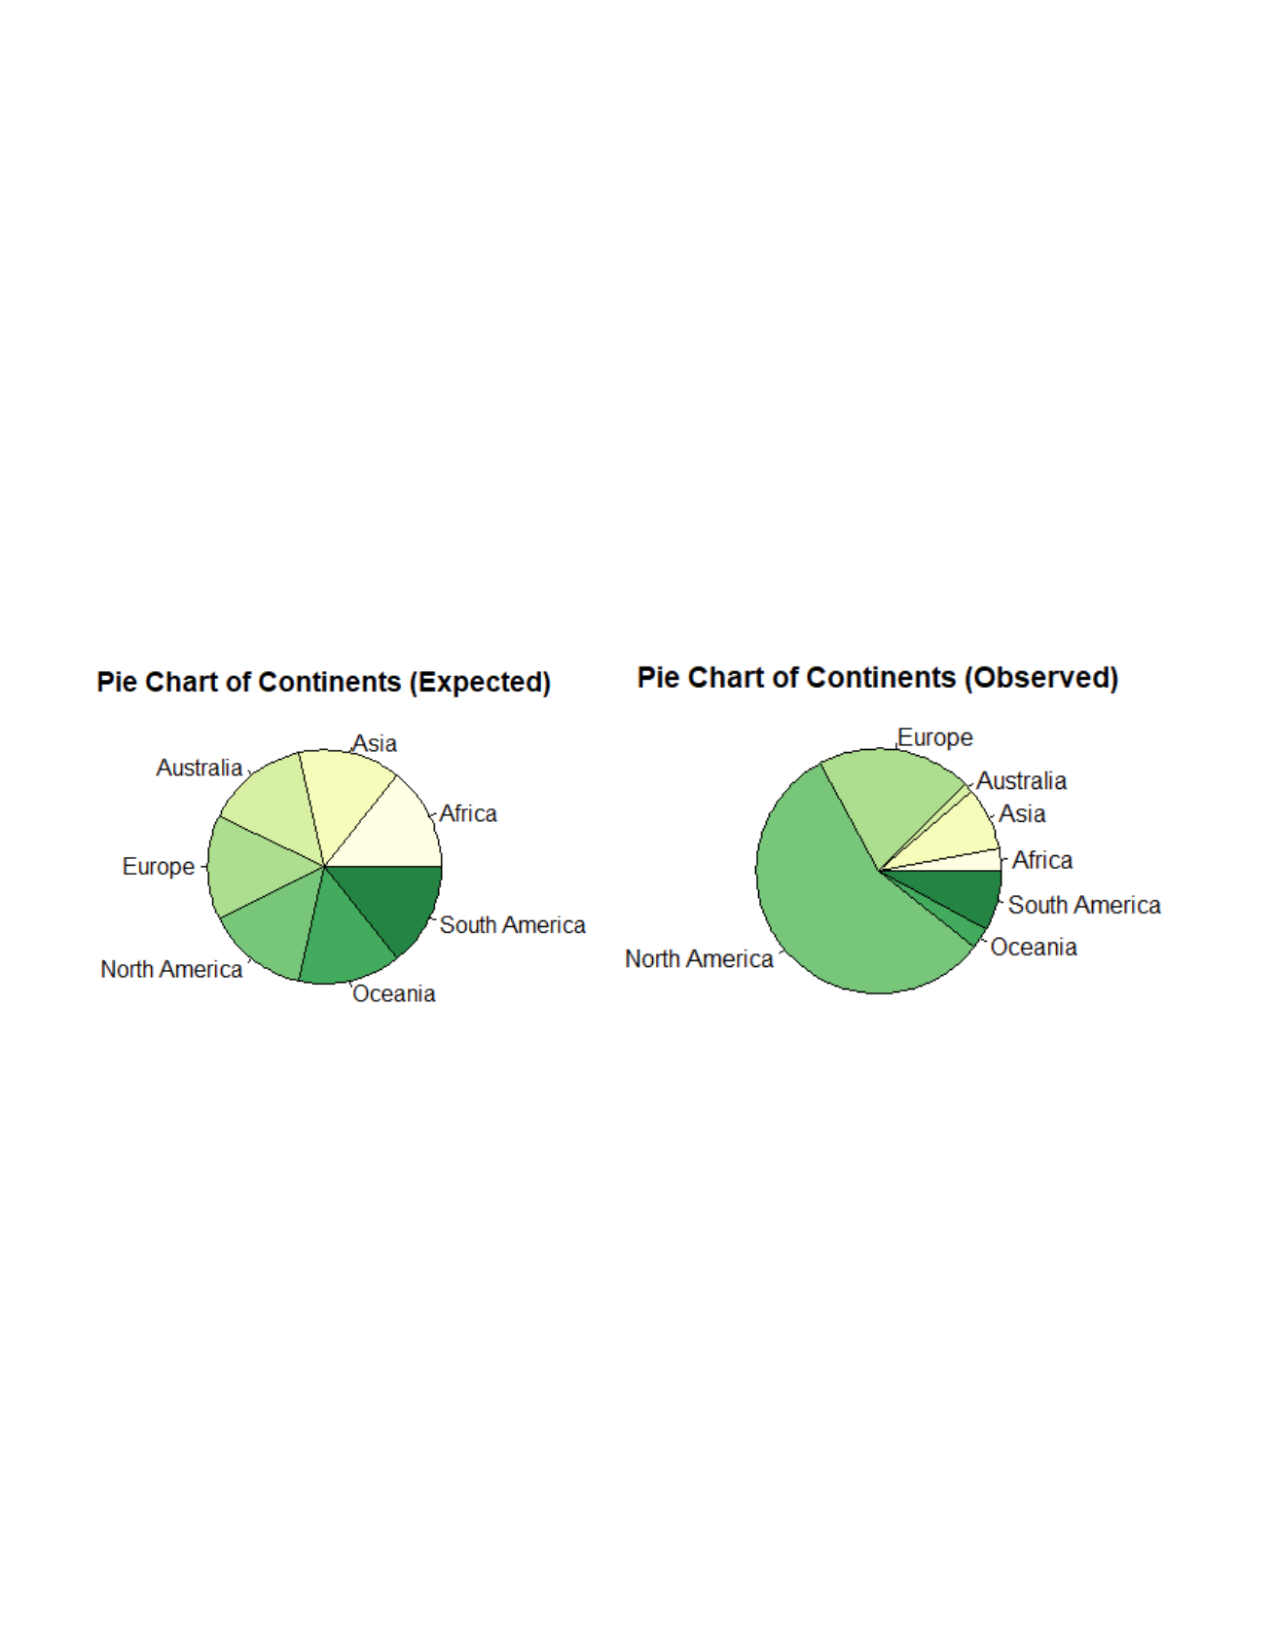
\includegraphics[width=0.50\textwidth]{ContinentPieChart.pdf}
    \label{fig:Continent Pie Chart}
\end{figure}

If the continents had a equal chance of being represented in these
published articles these pie charts would look similar. Unfortunately,
this is not the case and it is obvious that North America takes up the
majority of the pie chart.

If there is an assumption that the probability of each continent being
represented in a journal entry is the same as each continent's square
mileage. Then the continent with larger square mileage would have more
published articles than those continent with a smaller square mileage.
Below, is a XChi-Square test that shows if this statement is true or
not.

\begin{figure}
    \centering
    \includegraphics[width=0.50\textwidth]{ContinentChiSquare2i.pdf}
    \label{fig:Continent XChi-Square}
\end{figure}

Looking into the Pearson residuals notice that North America has the
most positive residual thus showing that the observed frequency exceeds
the expected frequency. Through visual representation, figure \emph{\#}
clarifies this idea. The bar graph on the left is the number of journals
one expects to see given each continent's square mileage. The bar graph
on the right is what was observed using the counts from the data set.

\begin{figure}
    \centering
>>>>>>> Stashed changes
    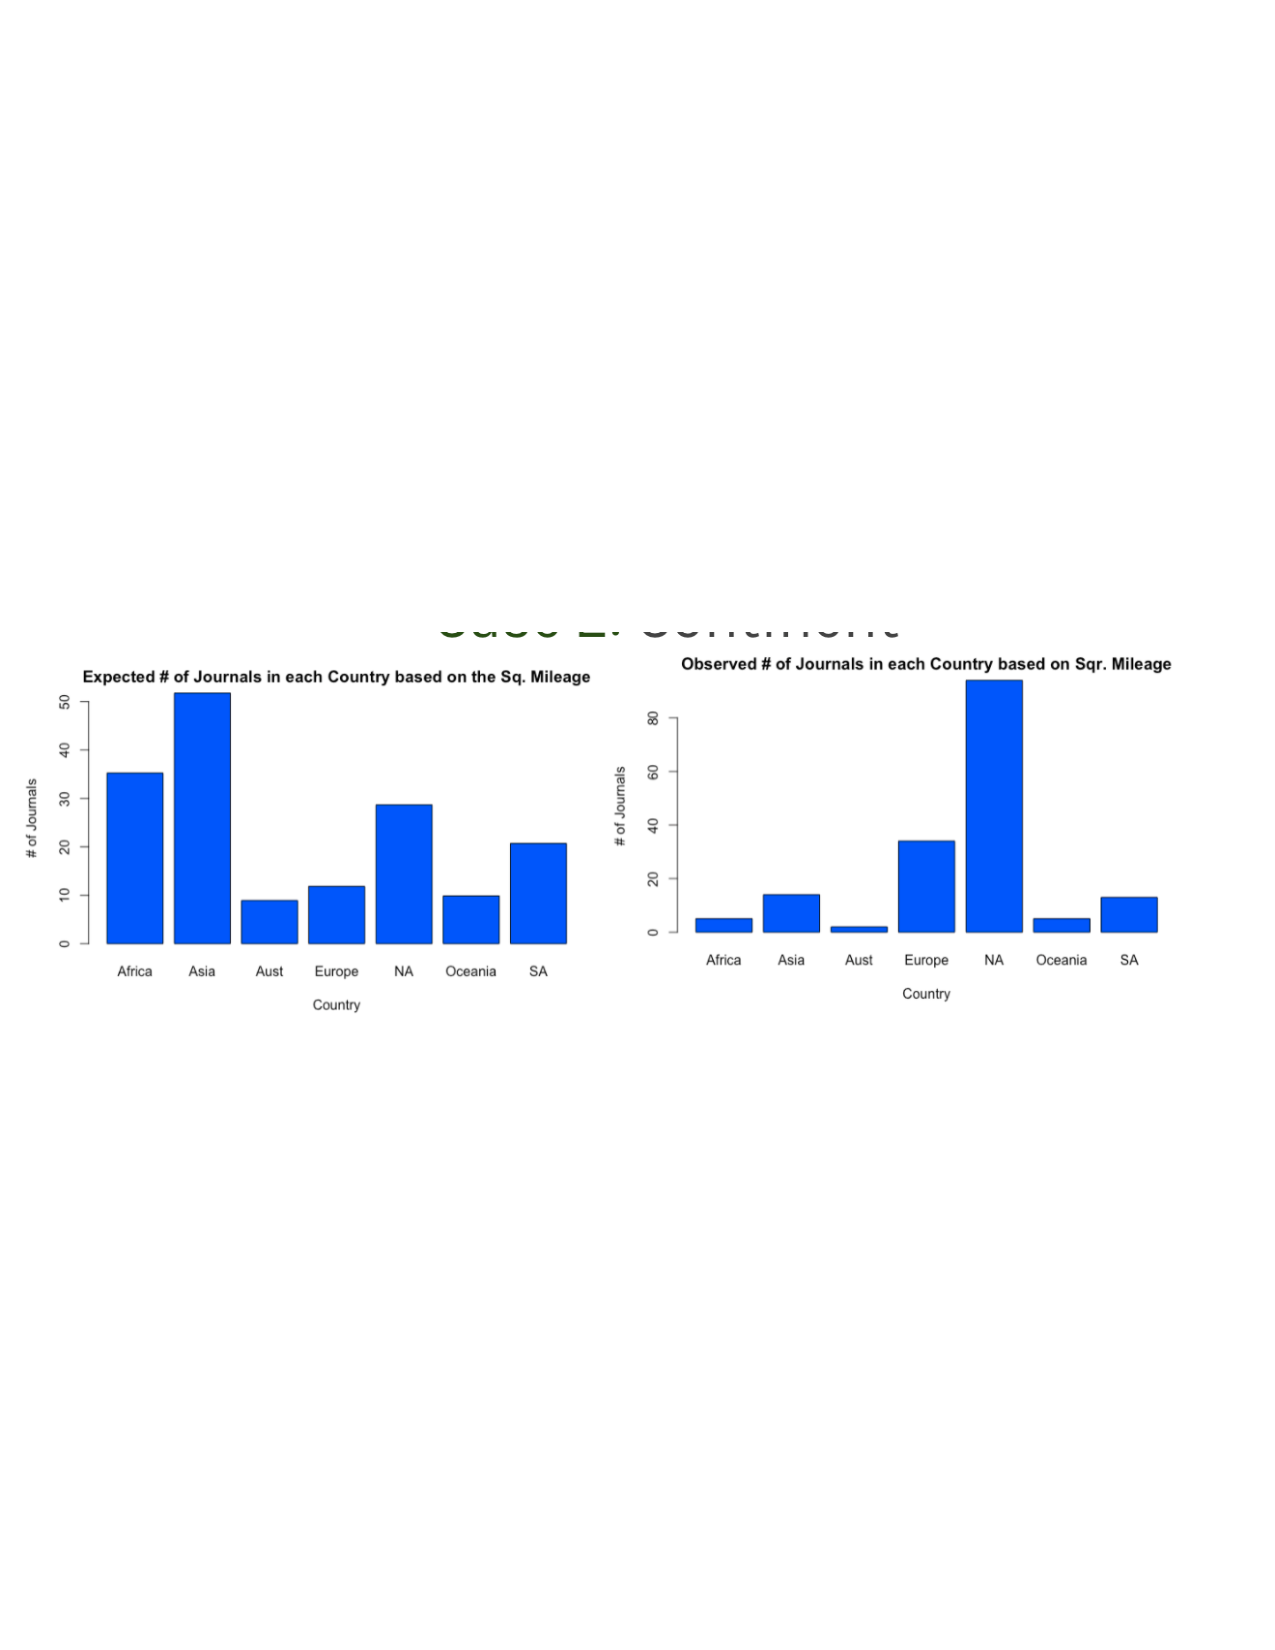
\includegraphics[width=0.50\textwidth]{Continent2BarGraph.pdf}
    \label{fig:Continent Bar Graph}
\end{figure}

Asia is the continent with the largest square mileage in comparison to
the other continents, and it has the largest number of expected journals
based on it's square mileage. However it resulted in being one of the
continent with the least number of journals based on the observed data.
Asia and every continent besides North America never met the assumption.
From the bar graph one can conclude that the probability of each
continent being represented in a journal entry is not the same as the
continents square mileage. In other words, giving that a continent is
larger does not mean there are more published articles from that
particular continent.

\hypertarget{b.-country}{%
\subsection{b. Country}\label{b.-country}}

The variable country accounted for how many of these published articles
completed the work done for the study in a particular country. Thus, we
can see how many published articles from this collection of data have
ecology work done in countries. To better model this, a contingency
table was made to depict how frequently work done in a particular
country was represented in the data set.

\begin{figure}
    \centering
    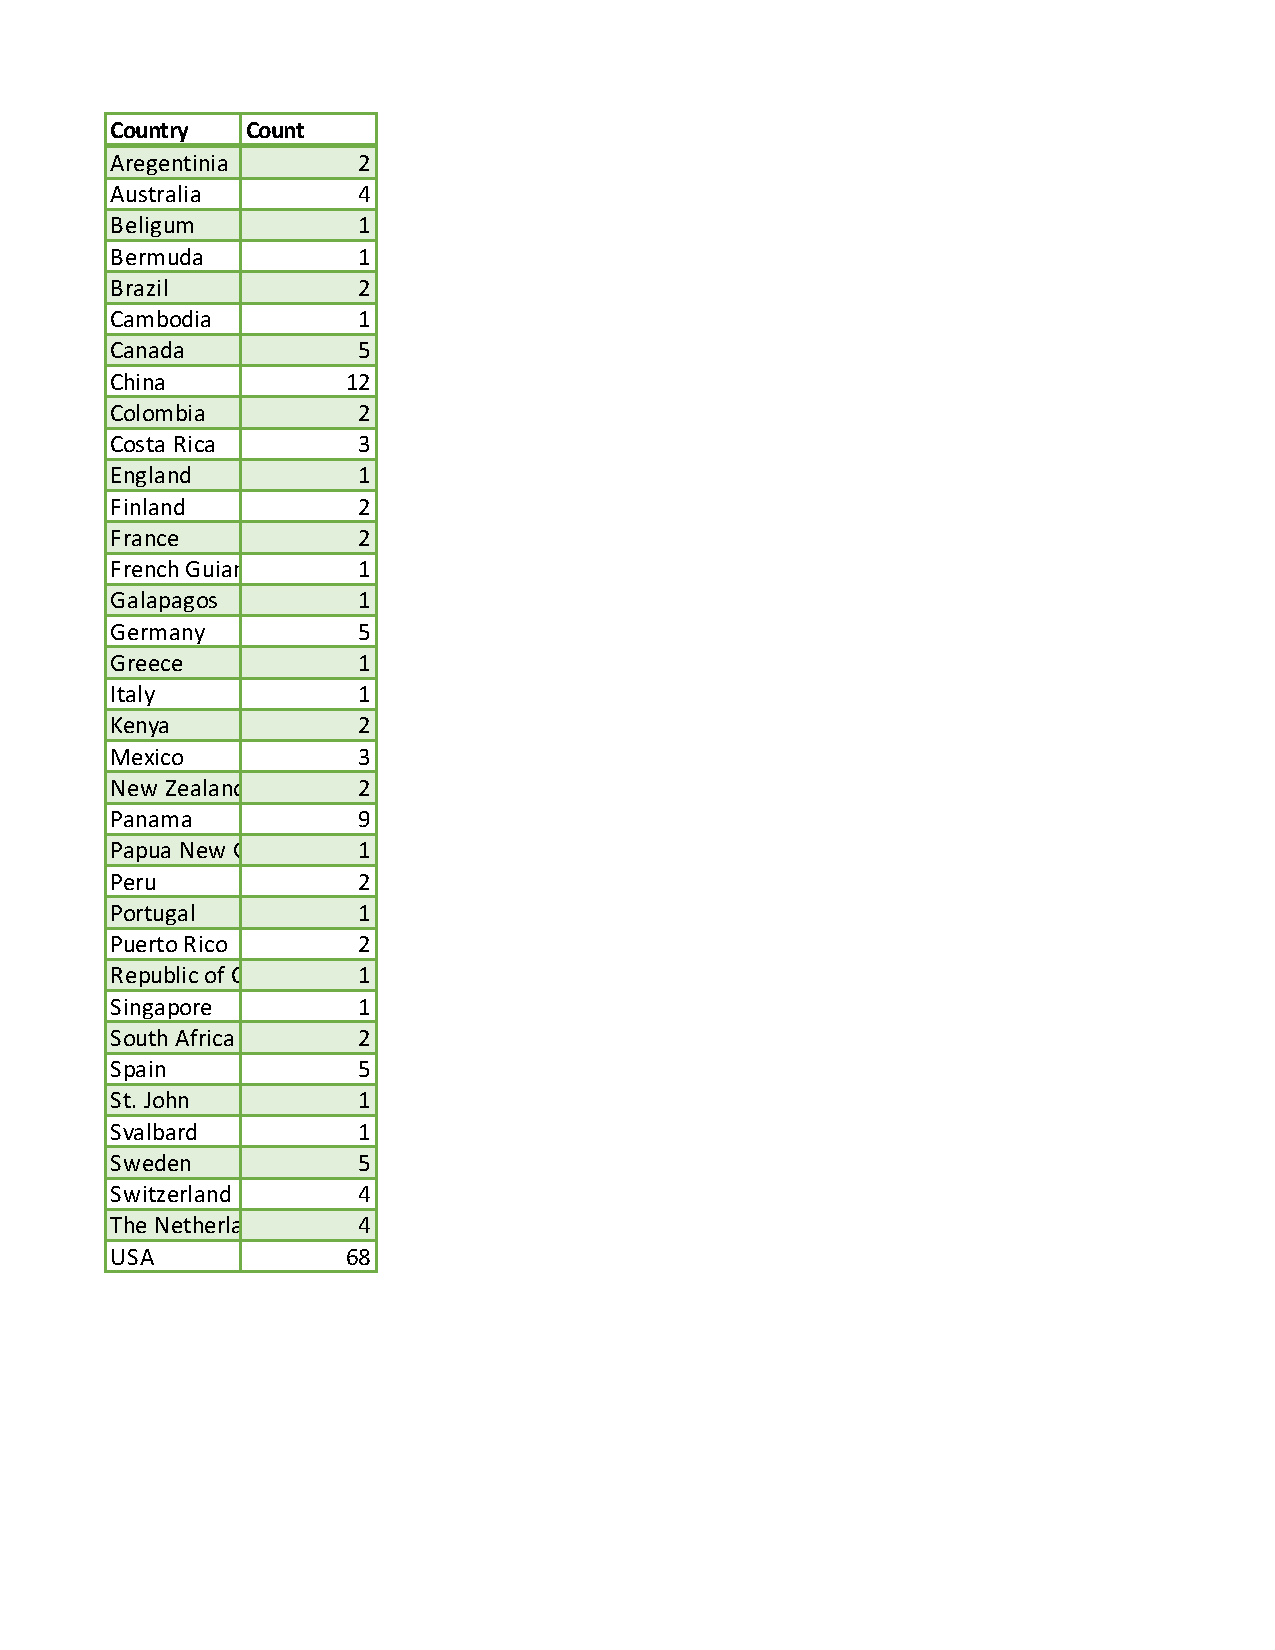
\includegraphics[width=0.50\textwidth]{country_contingency.pdf}
    \caption{This contingency table shows the frequency of countries in journal articles. Not all countries are represented because there were not journal articles that had work done in every country in the data set.}
    \label{fig:Contingency Table for Country}
\end{figure}

From the figure above, an be seen that the country where the study was
done, that had the highest frequency of articles was the United States.
There were 68 journal articles where the work was in the United States.
This is different from the number of articles with work done in other
countries, it was more common that each only had one or two journal
articles.

Using a chi squared test, we analyzed whether the probability of each
country being represented in a journal article is the same. This test
was run with the assumption that every country had an equal chance.

\begin{figure}
    \centering
    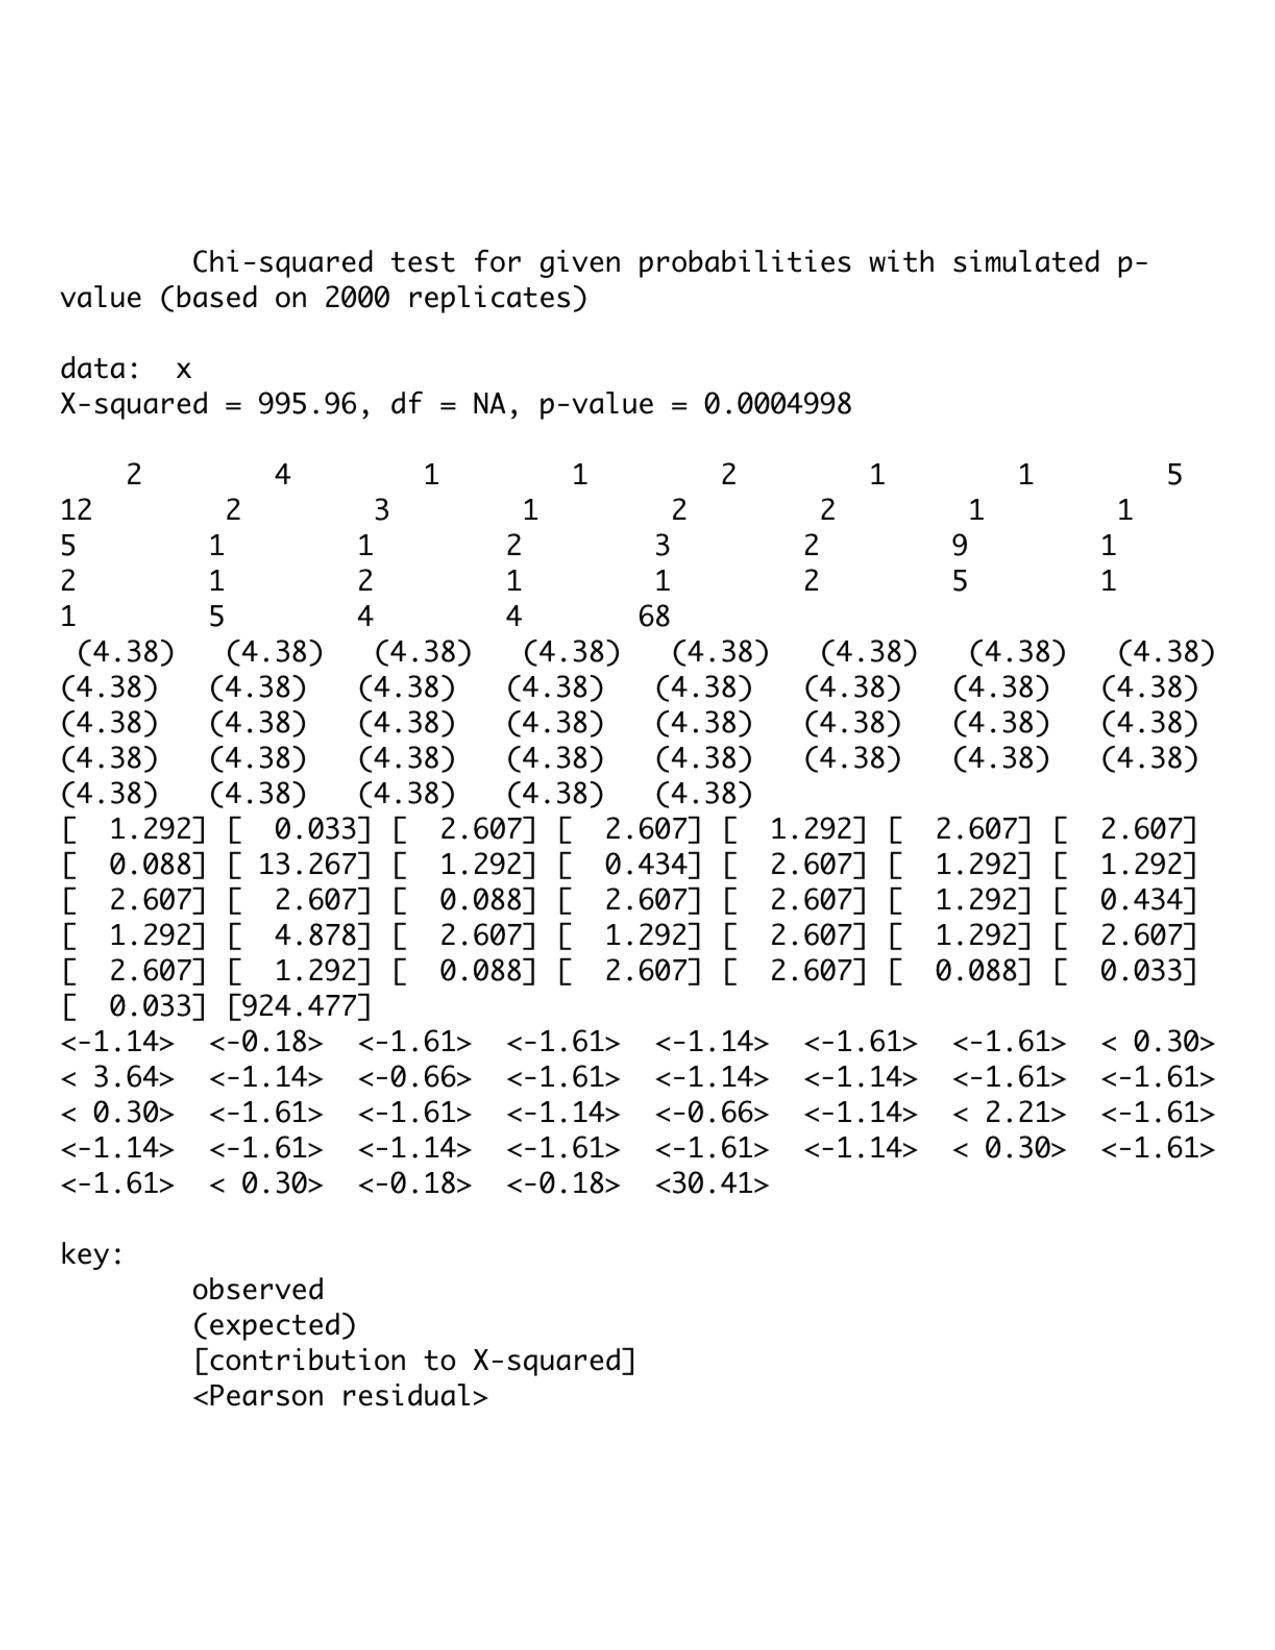
\includegraphics[width=0.50\textwidth]{xchisq_country.pdf}
    \caption{The xchi-square test above is analyzing whether the probability of each country in a  journal article is equal. The expected numer of journal articles for each country is approximately 4. The expected values are in parentheses and the observed values are just above it.}
    \label{fig:Chi Square for Country}
\end{figure}

From the figure above, the expected number of articles from each country
is approximately 4. Yet from the observed frequencies above, we can see
that many countries only have 1 or two articles with work done there,
but the United States has 68. Therefore, we can say that the probability
of each country being represented in a journal article might not be the
same.

Being that the size of each country varies, it would not make sense for
each country to have the same likelihood of being represented in a
journal article. Thus, the square mileage of each country was researched
in order to better estimate the probability of each country being
represented in a journal article.

\hypertarget{c.-region}{%
\subsection{c.~Region}\label{c.-region}}

The region category exhibited if any or the amount of published articles
completed their study in a particular region. This allowed us to see
which region were more or less commonly seen for ecology work. The
following contingency table counts the number of times a region was
represented in the data set.

\begin{figure}
    \centering
    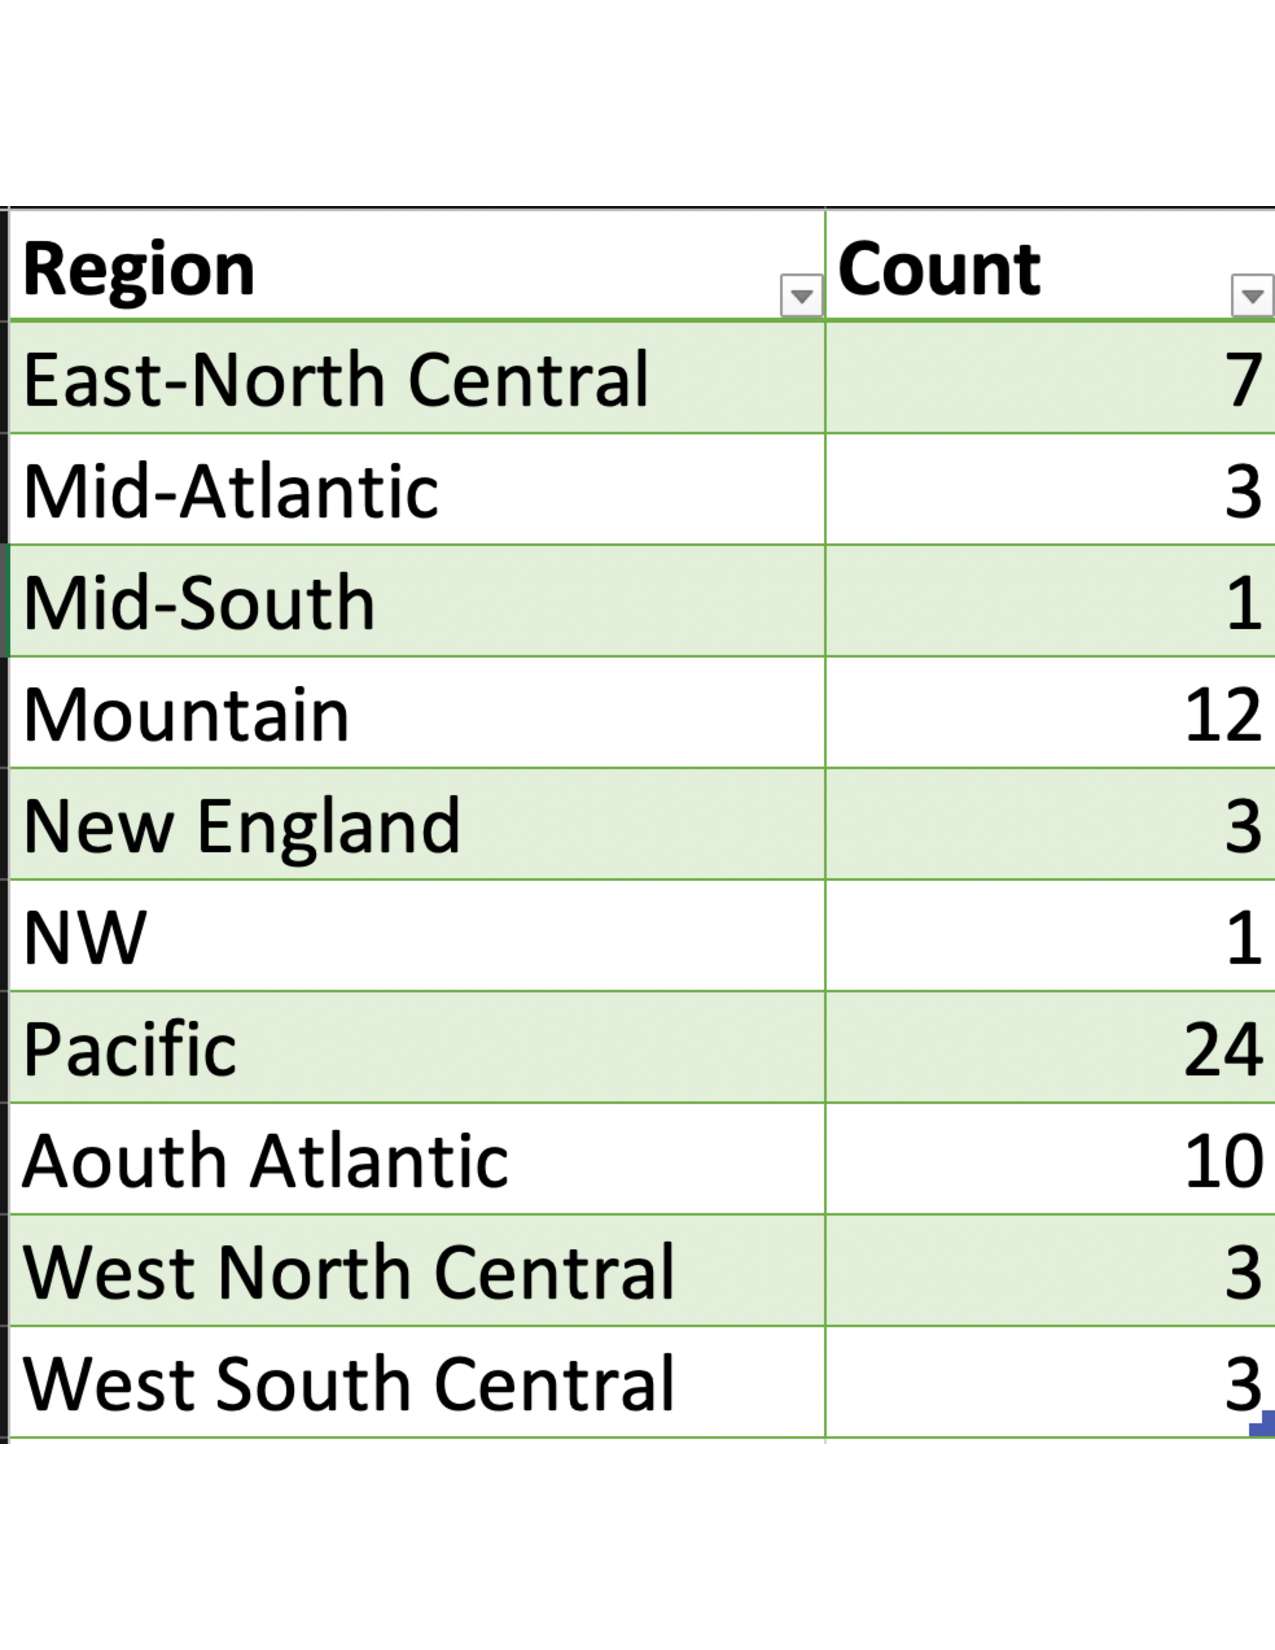
\includegraphics[width=0.50\textwidth]{RegionsContingencyTable.pdf}
    \label{fig:Contingency Table}
\end{figure}

From the table above notice the number of published articles is higher
in the Pacific region in comparison to the other regions.

If there is an assumption that the probability of each region being
represented in a journal entry is the same, then there should be the
same number of counts for each region. Below, is a XChi-Square test that
shows if this statement is true or not.

\begin{figure}
    \centering
    \includegraphics[width=0.50\textwidth]{RegionsChiSquare1.pdf}
    \label{fig:Region XChi-Square}
\end{figure}

From the Pearson residuals notice that Pacific has the most positive
residual thus, the observed frequency exceeds the expected frequency.
Additionally, Mid-South and North West has the most negative residual
thus, the observed frequency does not meet the expected frequency.
Through visual representation, figure \emph{\#} clarifies this idea. The
pie chart on the left shows what the pie chart should look like if every
region had an equal chance of being represented in a published article.
While the pie chart on the right is what the pie chart looks like when
using the counts from the data set.

\begin{figure}
    \centering
    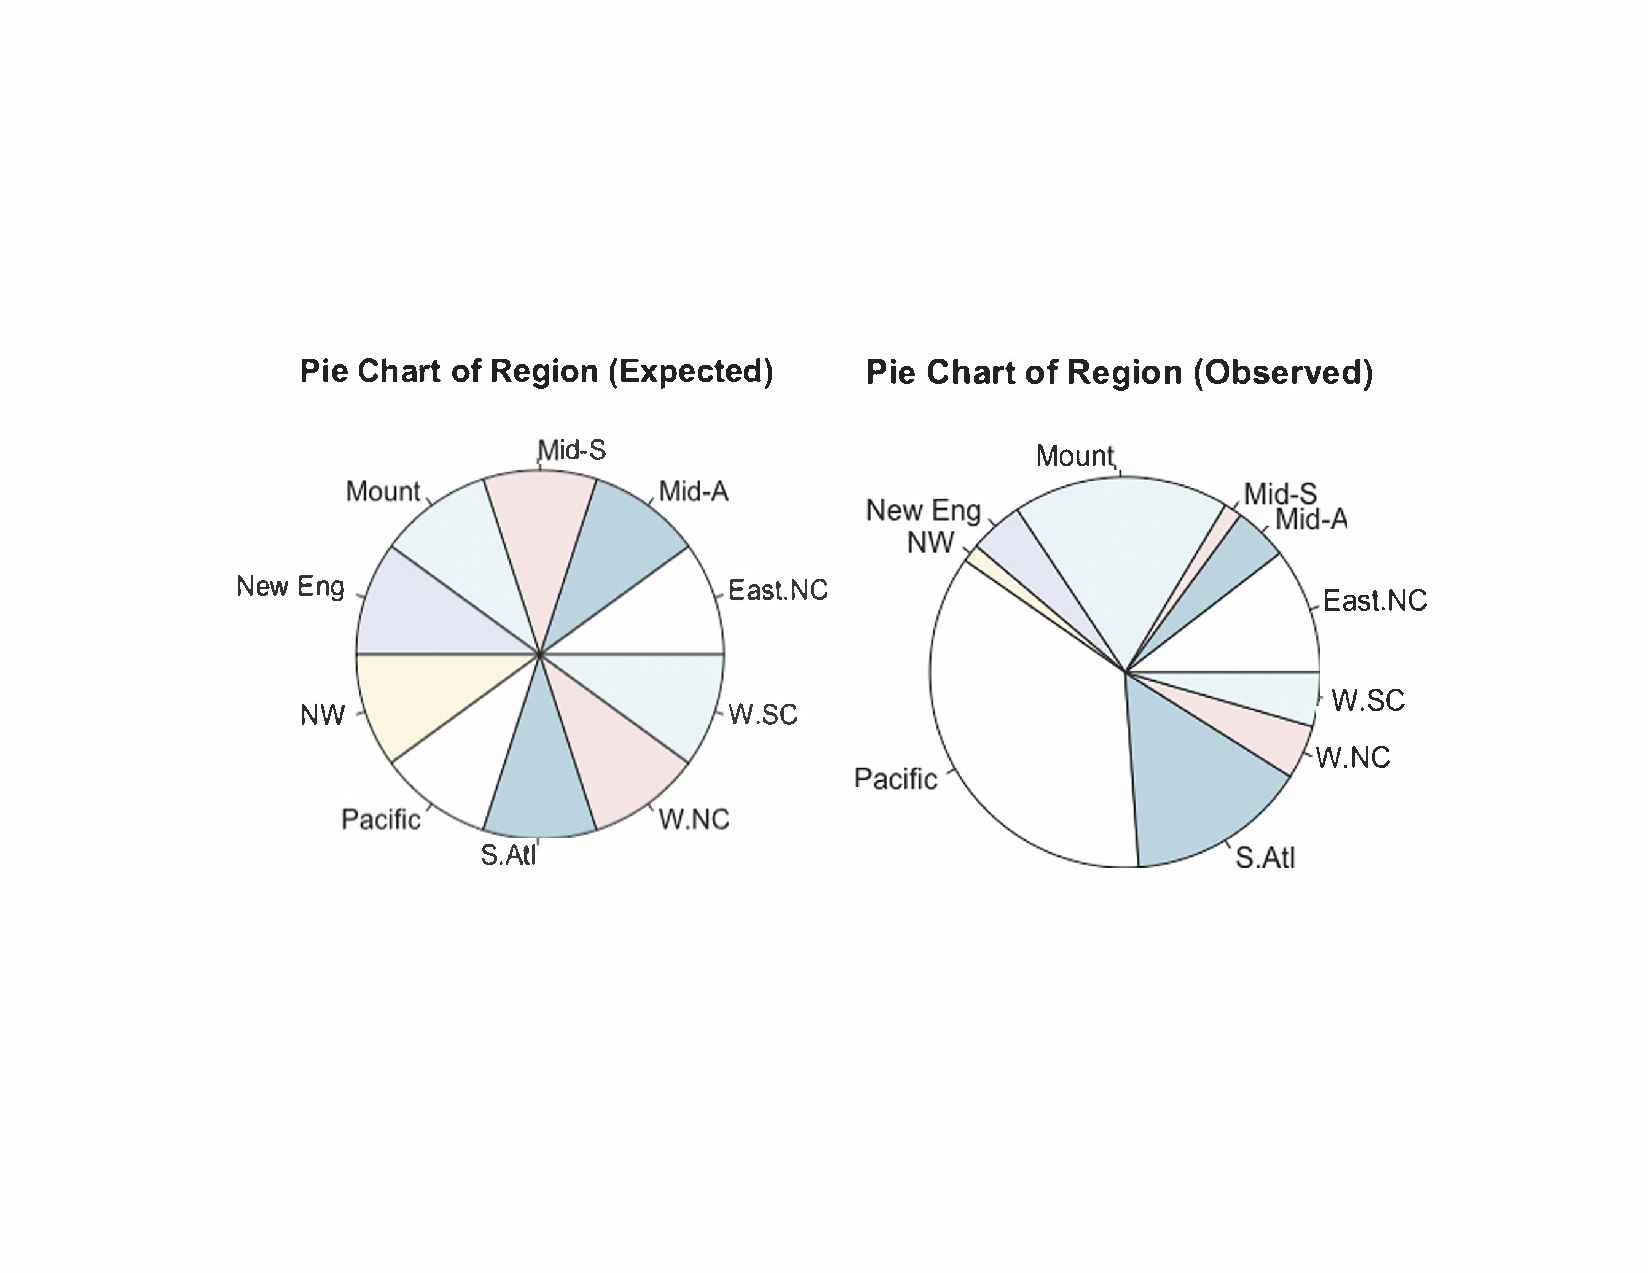
\includegraphics[width=0.50\textwidth]{RegionsPieChart.pdf}
    \label{fig:Region Pie Chart}
\end{figure}

If the regions had a equal chance of being represented in these
published articles these pie charts would look similar. Unfortunately,
this is not the case and it is obvious that Pacific takes up the
majority of the pie chart.

If there is an assumption that the probability of each region being
represented in a journal entry is the same as each region's square
mileage/ Then the region with a larger square mileage would have more
published articles than those regions with a smaller square mileage.
Below, is a Chi-Square test that shows if this statement is true or not.

\begin{figure}
    \centering
    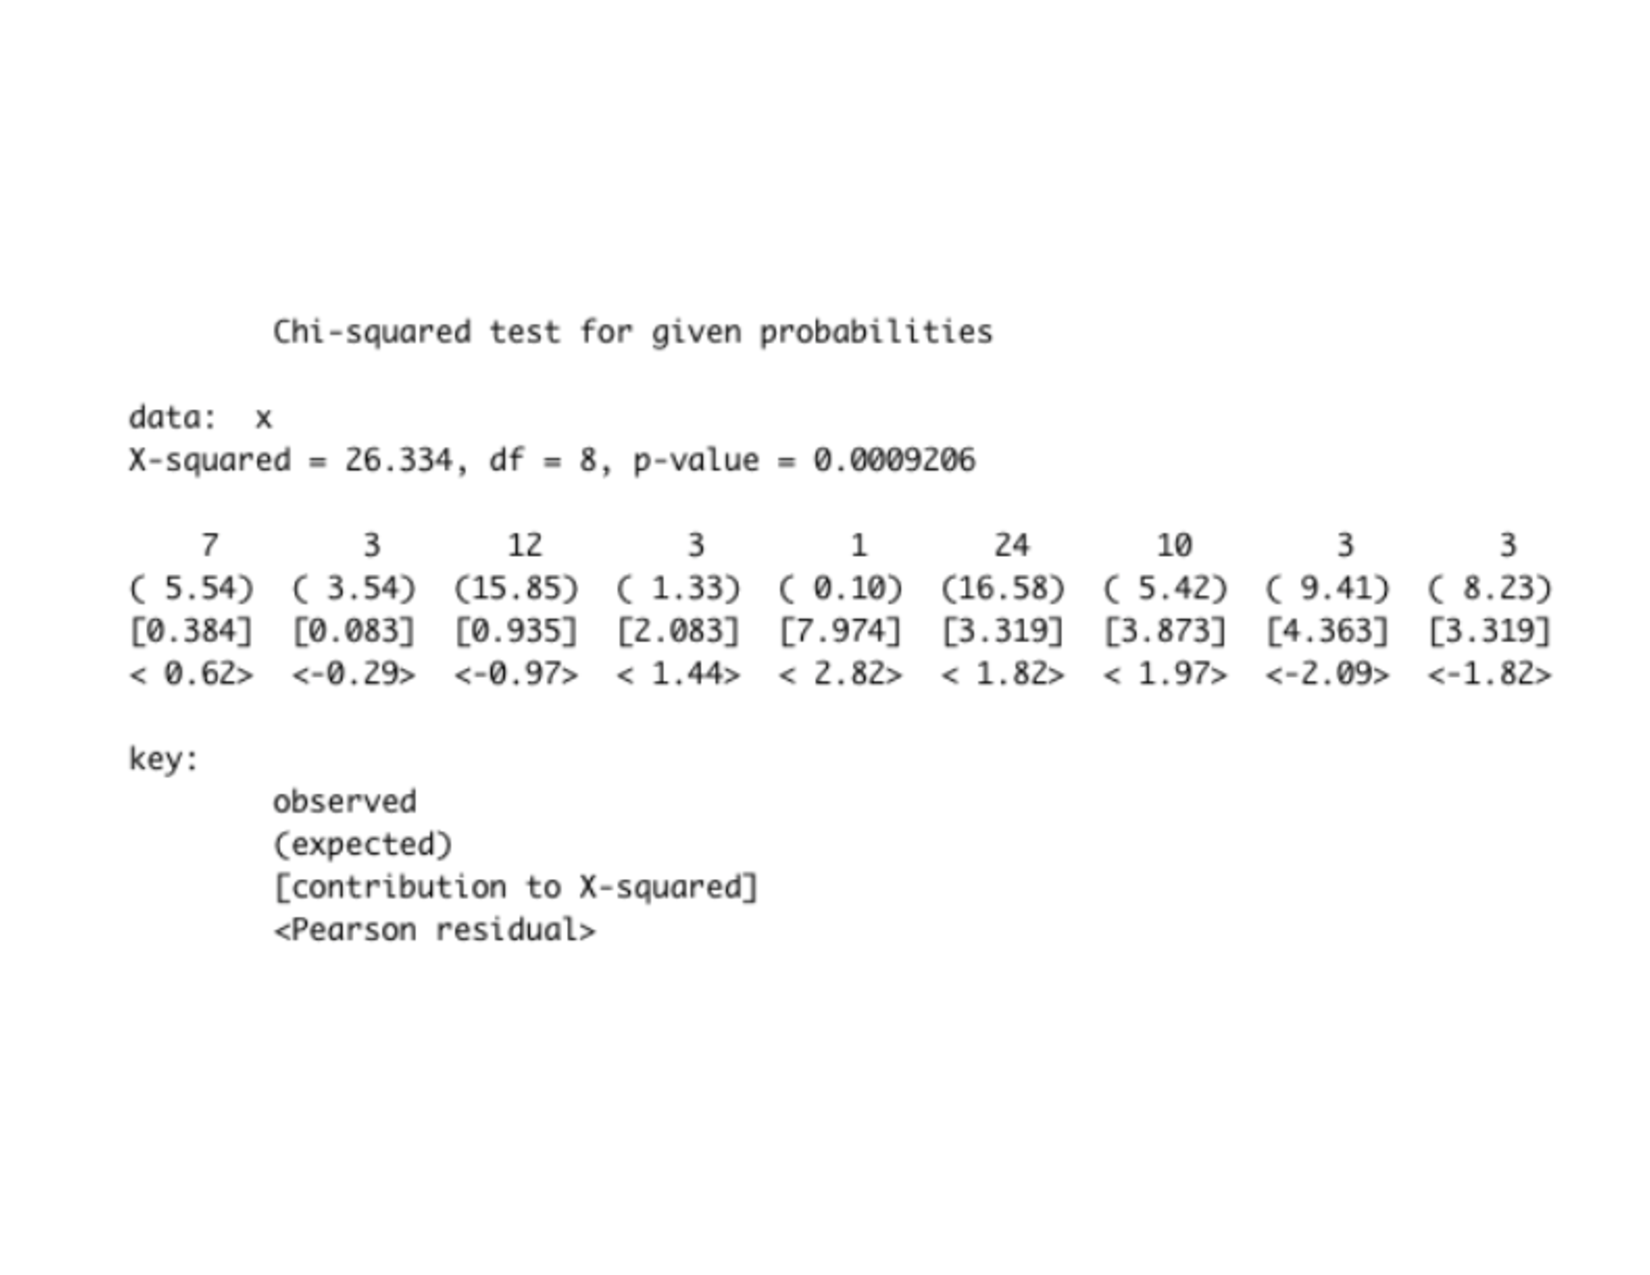
\includegraphics[width=0.50\textwidth]{RegionChiSquare2.pdf}
    \label{fig:Region XChi-Square}
\end{figure}

\begin{quote}
\begin{quote}
\begin{quote}
\begin{quote}
\begin{quote}
\begin{quote}
\begin{quote}
Stashed changes
\end{quote}
\end{quote}
\end{quote}
\end{quote}
\end{quote}
\end{quote}
\end{quote}

Looking into the Pearson residuals notice that North West has the most
positive residula this showing that the observed frequency exceeds the
expected frequency.

\hypertarget{c.-region-1}{%
\subsection{c.~Region}\label{c.-region-1}}

The region category exhibited if any or the amount of published articles
completed their study in a particular region. This allowed us to see
which region were more or less commonly seen for ecology work. The
following contingency table counts the number of times a region was
represented in the data set.

\begin{figure}
    \centering
    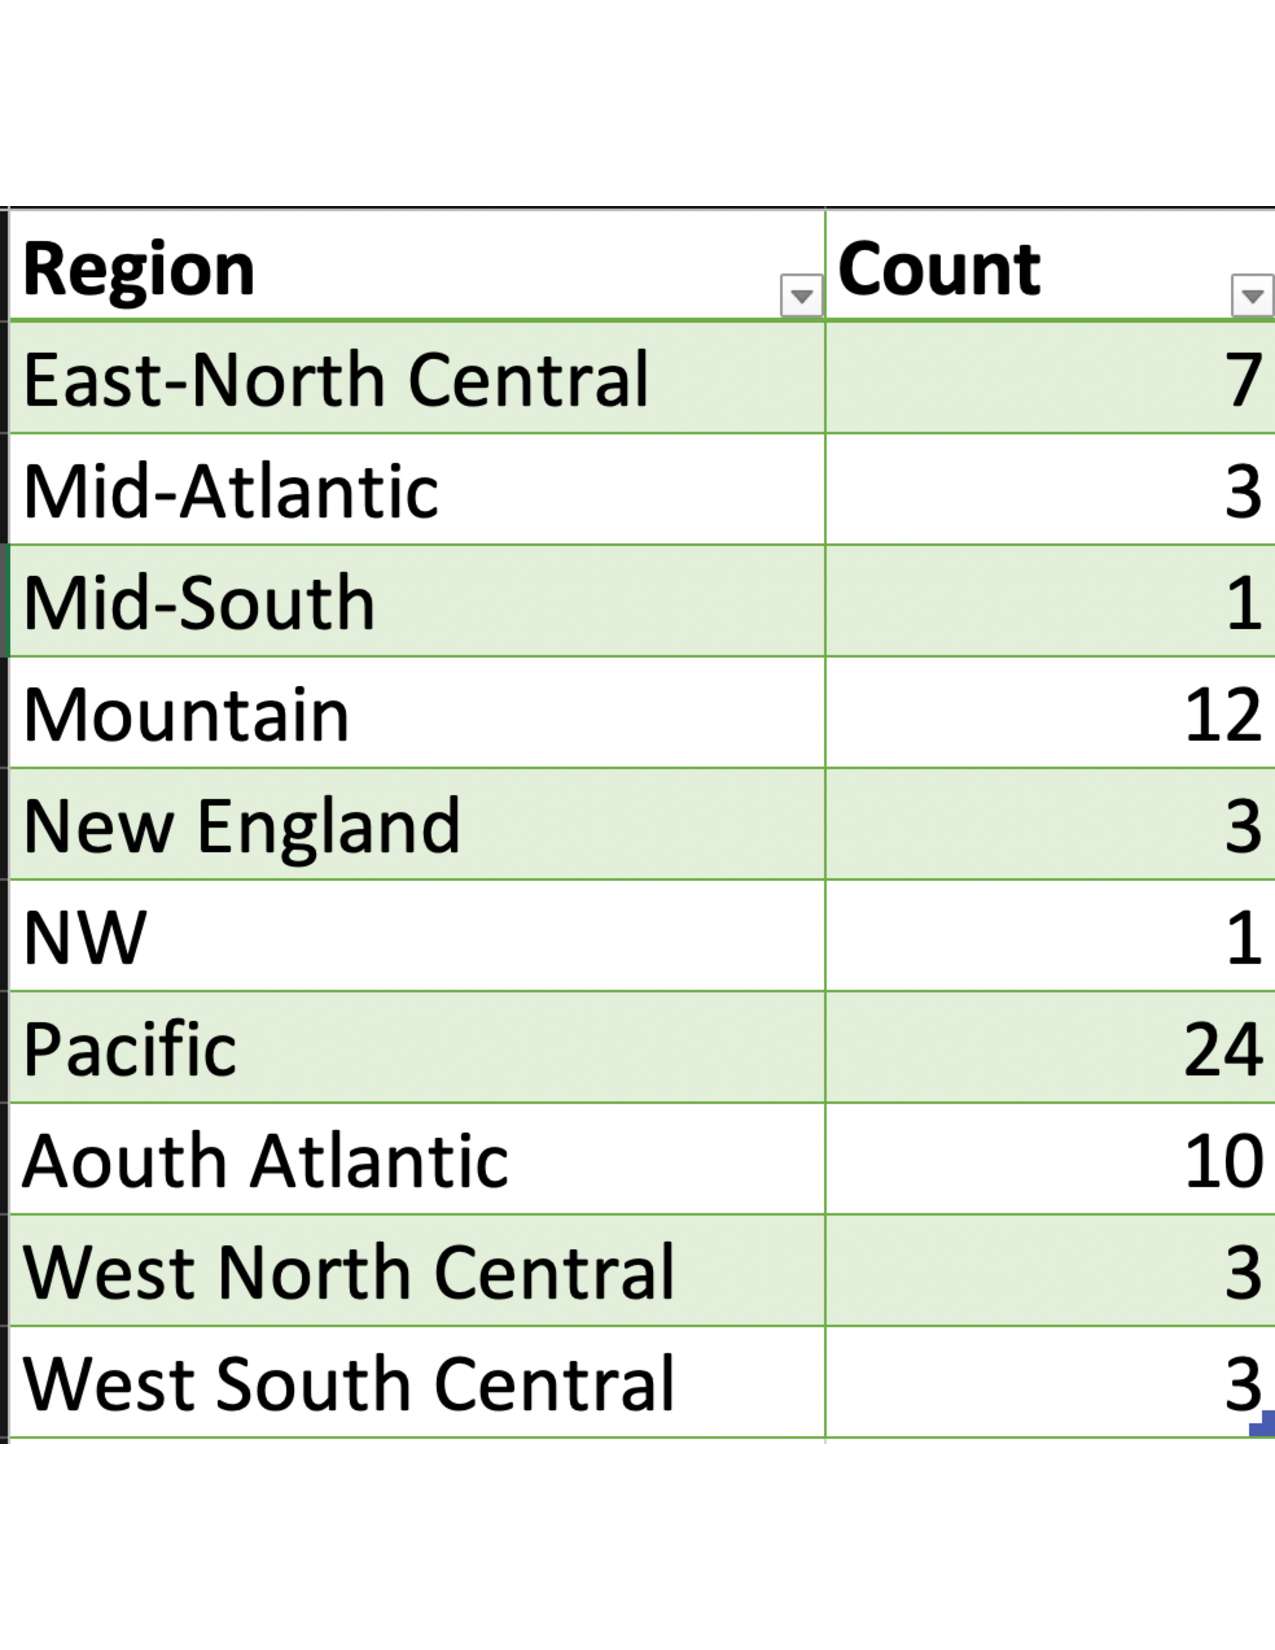
\includegraphics[width=0.50\textwidth]{RegionsContingencyTable.pdf}
    \label{fig:Contingency Table}
\end{figure}

From the table above notice the number of published articles is higher
in the Pacific region in comparison to the other regions.

If there is an assumption that the probability of each region being
represented in a journal entry is the same, then there should be the
same number of counts for each region. Below, is a XChi-Square test that
shows if this statement is true or not.

\begin{figure}
    \centering
    \includegraphics[width=0.50\textwidth]{RegionsChiSquare1.pdf}
    \label{fig:Region XChi-Square}
\end{figure}

From the Pearson residuals notice that Pacific has the most positive
residual thus, the observed frequency exceeds the expected frequency.
Additionally, Mid-South and North West has the most negative residual
thus, the observed frequency does not meet the expected frequency.
Through visual representation, figure \emph{\#} clarifies this idea. The
pie chart on the left shows what the pie chart should look like if every
region had an equal chance of being represented in a published article.
While the pie chart on the right is what the pie chart looks like when
using the counts from the data set.

\begin{figure}
    \centering
    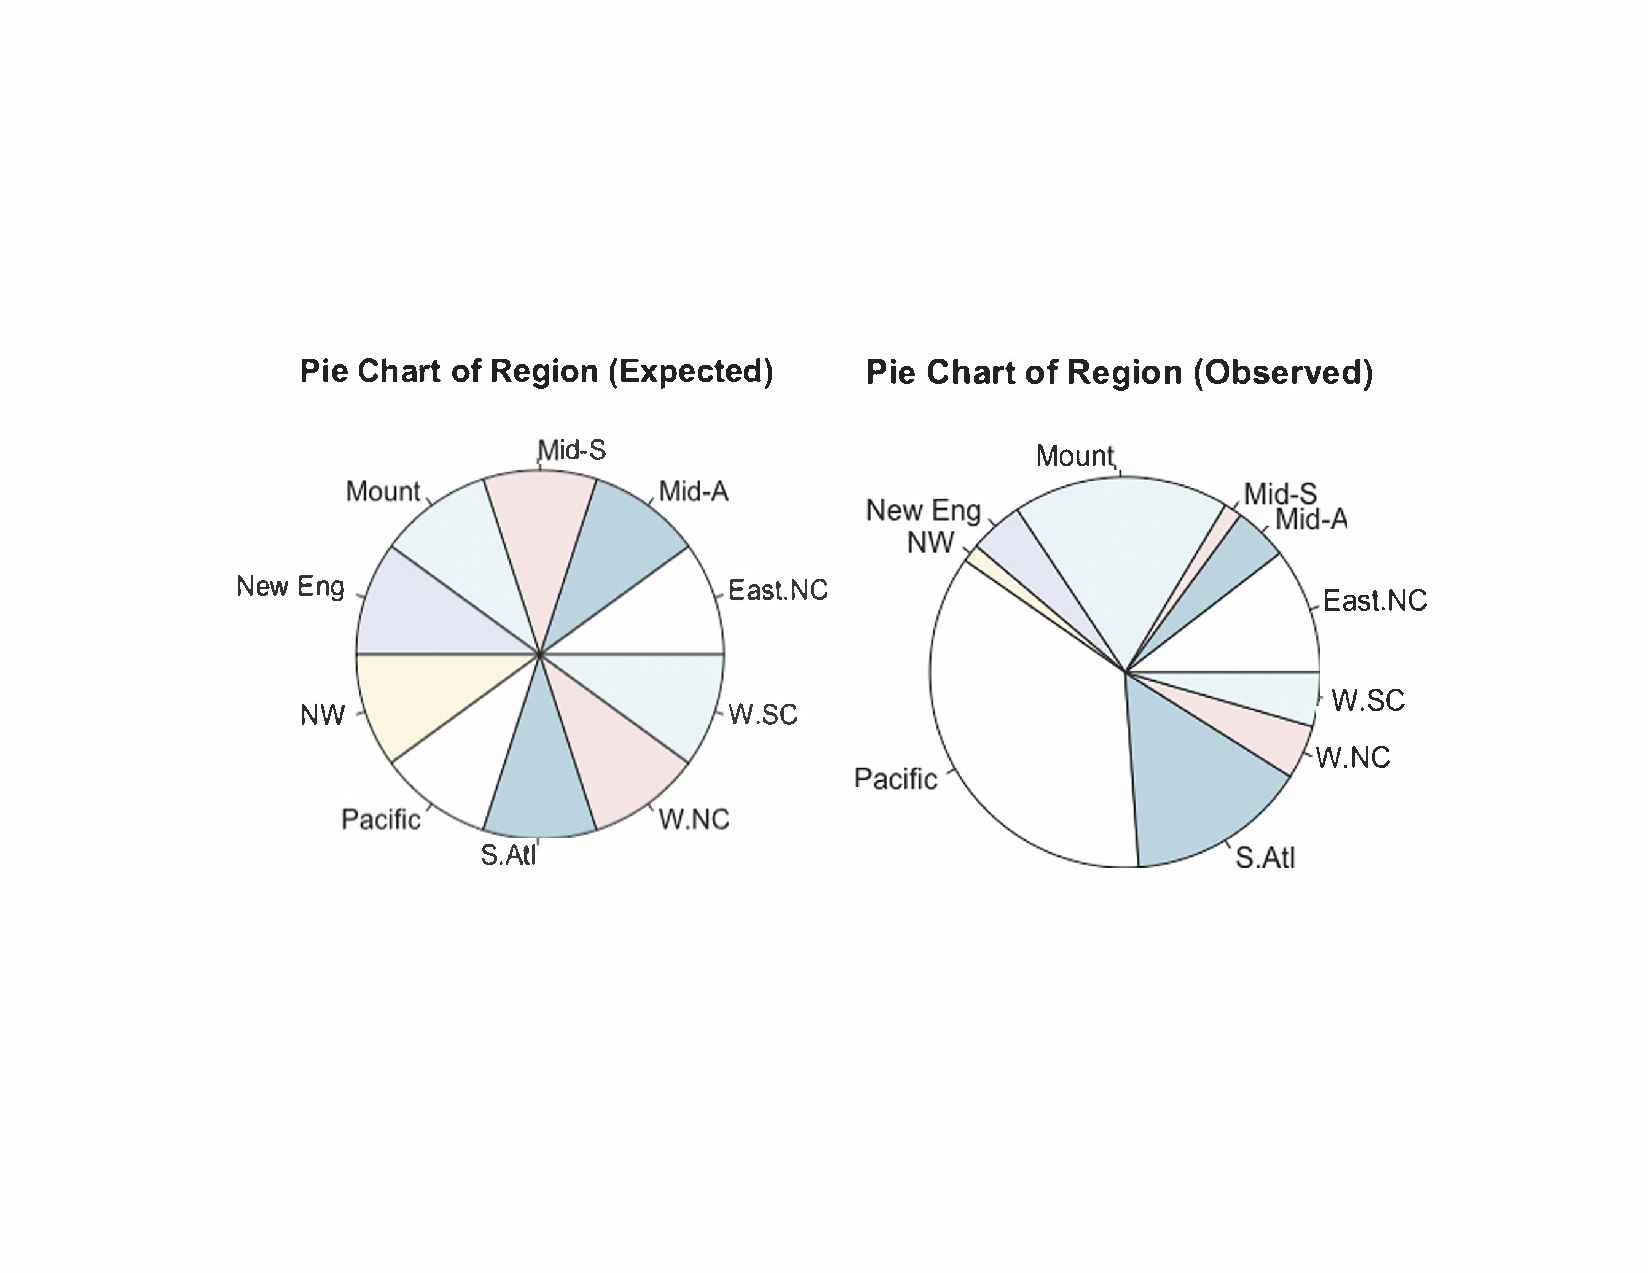
\includegraphics[width=0.50\textwidth]{RegionsPieChart.pdf}
    \label{fig:Region Pie Chart}
\end{figure}

If the regions had a equal chance of being represented in these
published articles these pie charts would look similar. Unfortunately,
this is not the case and it is obvious that Pacific takes up the
majority of the pie chart.

If there is an assumption that the probability of each region being
represented in a journal entry is the same as each region's square
mileage/ Then the region with a larger square mileage would have more
published articles than those regions with a smaller square mileage.
Below, is a Chi-Square test that shows if this statement is true or not.

\begin{figure}
    \centering
    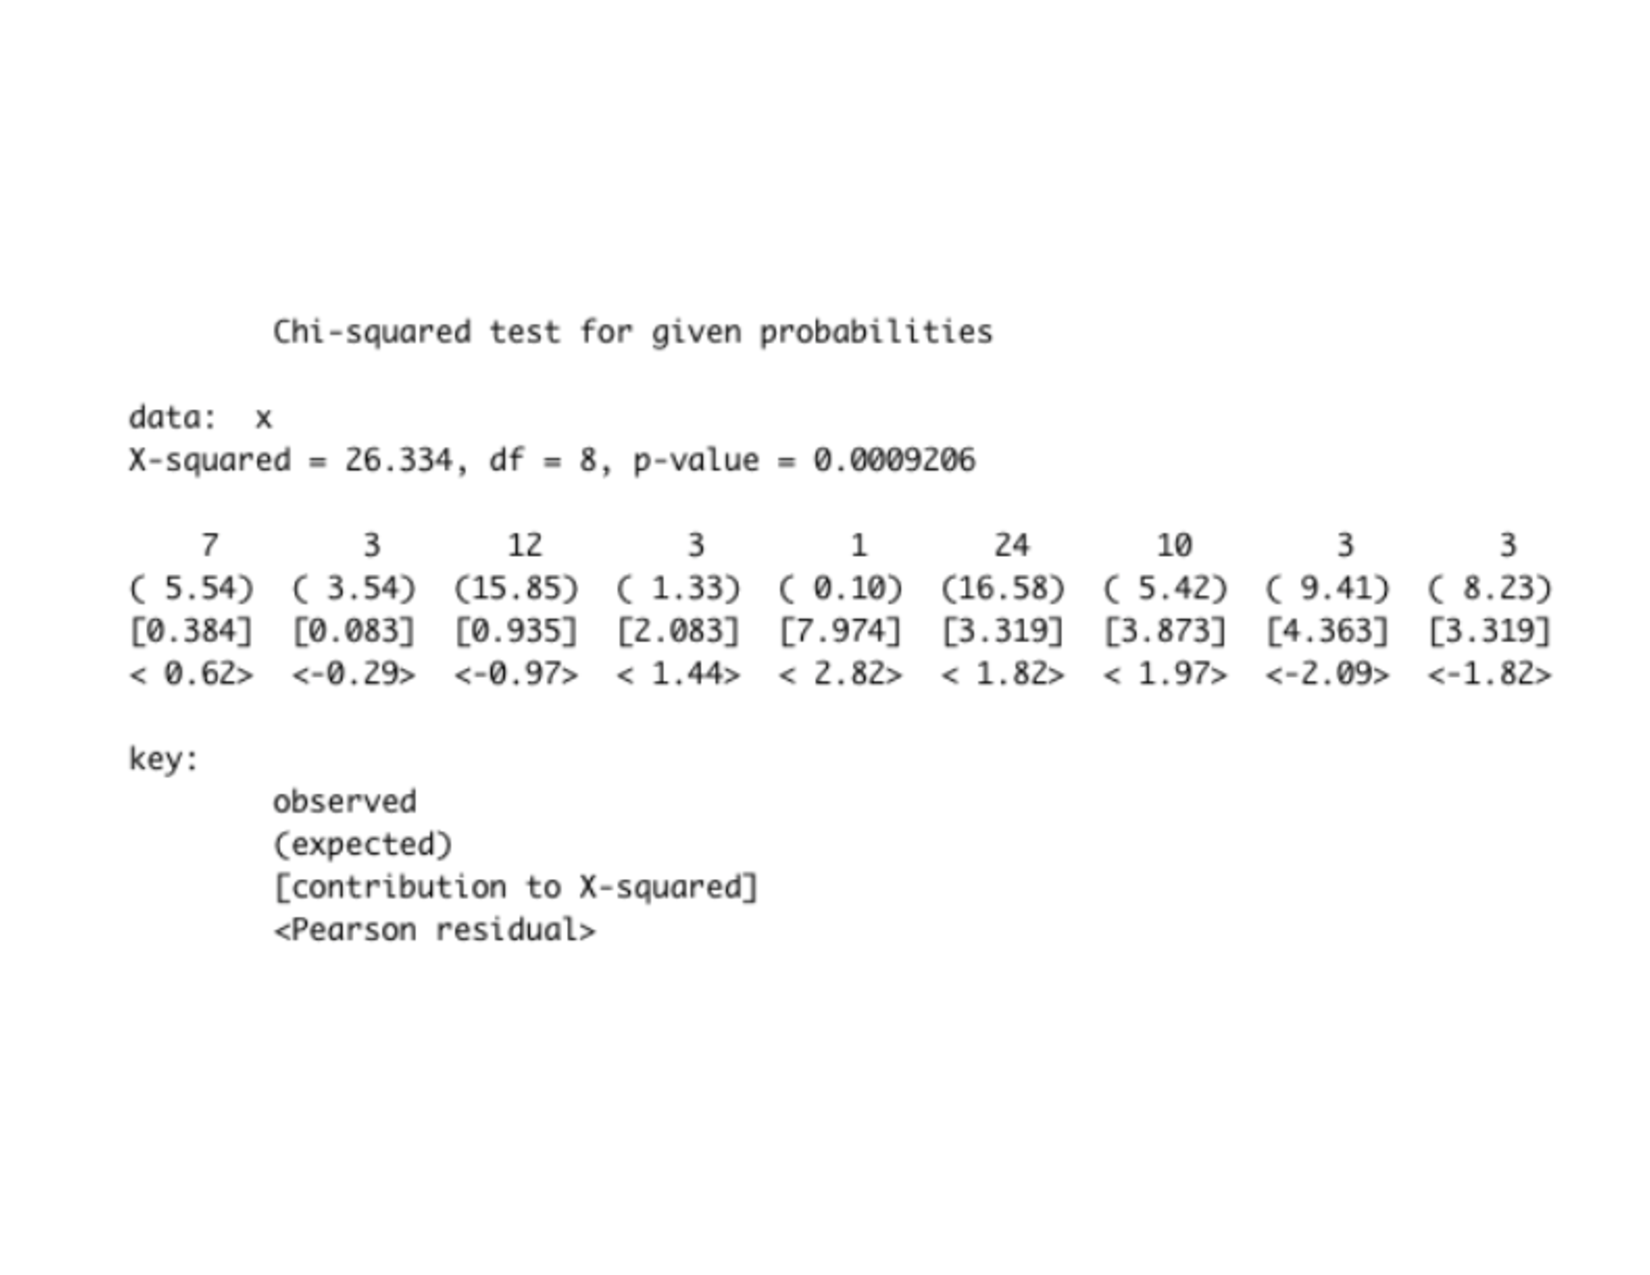
\includegraphics[width=0.50\textwidth]{RegionChiSquare2.pdf}
    \label{fig:Region XChi-Square}
\end{figure}

Looking into the Pearson residuals notice that North West has the most
positive residual thus showing that the observed frequency exceeds the
expected frequency. Through visual representation, figure \emph{\#}
clarifies this idea. The bar graph on the left is the number of journals
one expects to see given each region's square mileage. The bar graph on
the right is what was observed using the counts from the data set. Also,
due to unidentifiable region we couldn't locate square mileage for
Mid-South. Due to this, we redid some data cleaning to remove this
region. So our results do not include this specific region.

\begin{figure}
    \centering
    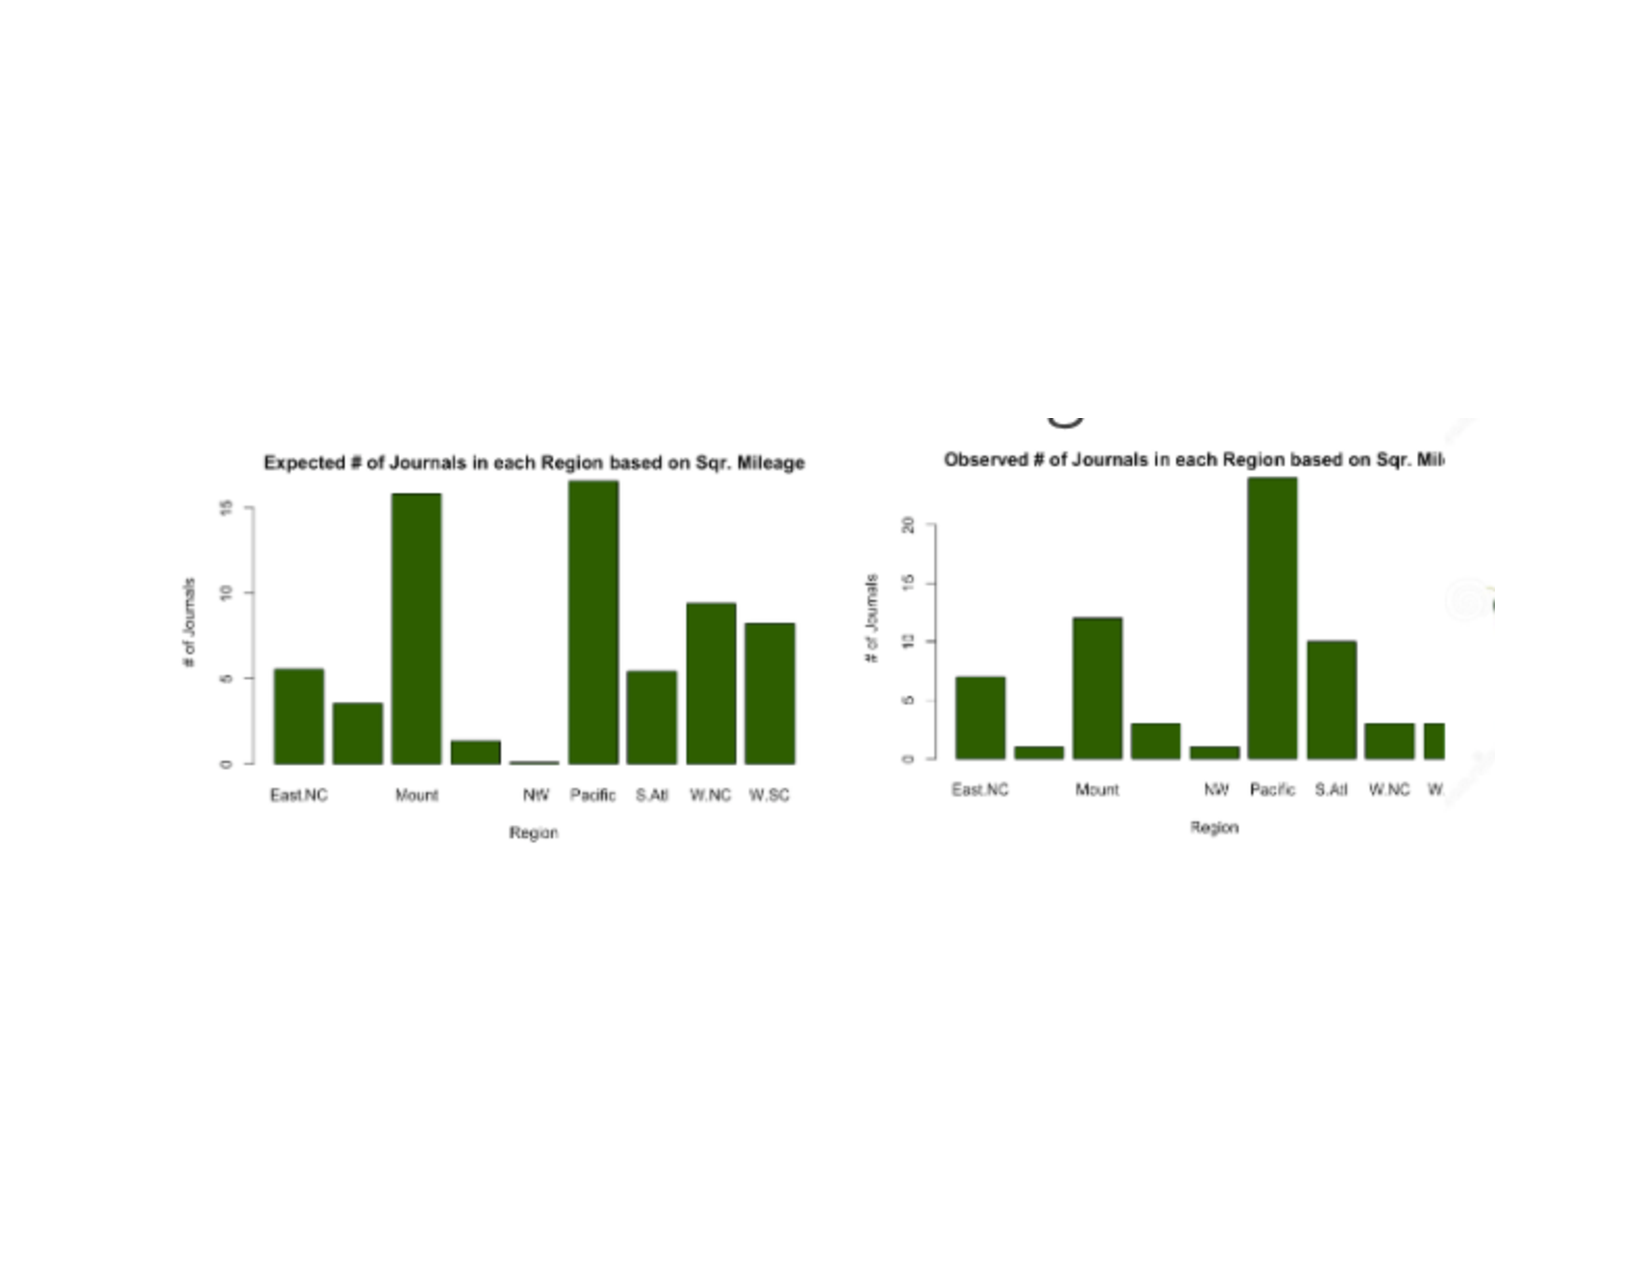
\includegraphics[width=0.50\textwidth]{Regions2BarGraph.pdf}
    \label{fig:Continent Bar Graph}
\end{figure}

\hypertarget{d.-state}{%
\subsection{d.~State}\label{d.-state}}

The state category noted if and how many of these published articles
completed their study in a particular state. This allowed us to see
which states were more or less popular for ecology work. The following
contingency table counts the number of times a state was represented in
the data set.

\begin{figure}
  \caption{Contingency Table}
    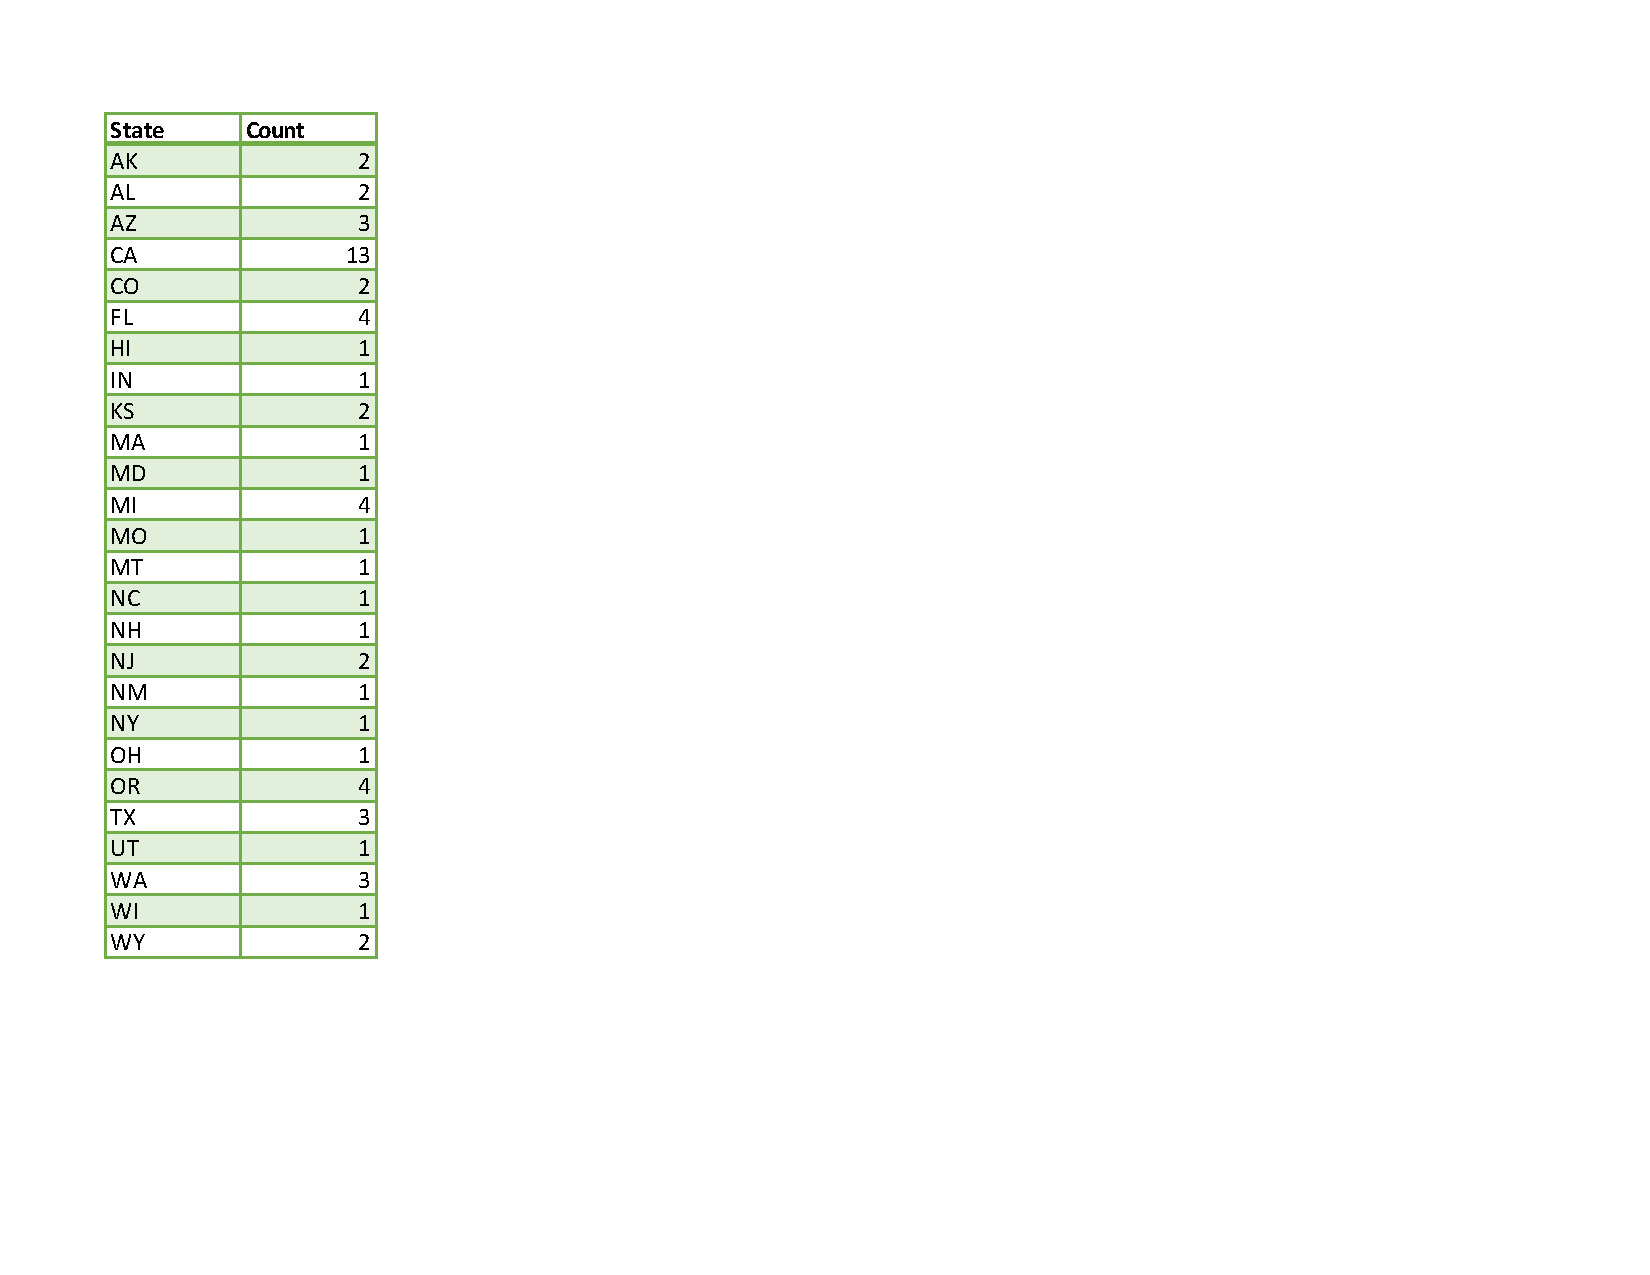
\includegraphics[width=13cm]{statetable.pdf}
\end{figure}

From the table above, one can tell that most of the journal entries are
published when the work was in California. The states that are not
included in the table were never represented in the data set. If there
is an assumption that the probability of each state being represented in
a journal entry is the same as each state's square mileage then the
larger states would have more published articles than the smaller
states. Below, is the Chi-Square test that test if this statement is
true.

\begin{figure}
  \caption{Chi-Square Test: States}
    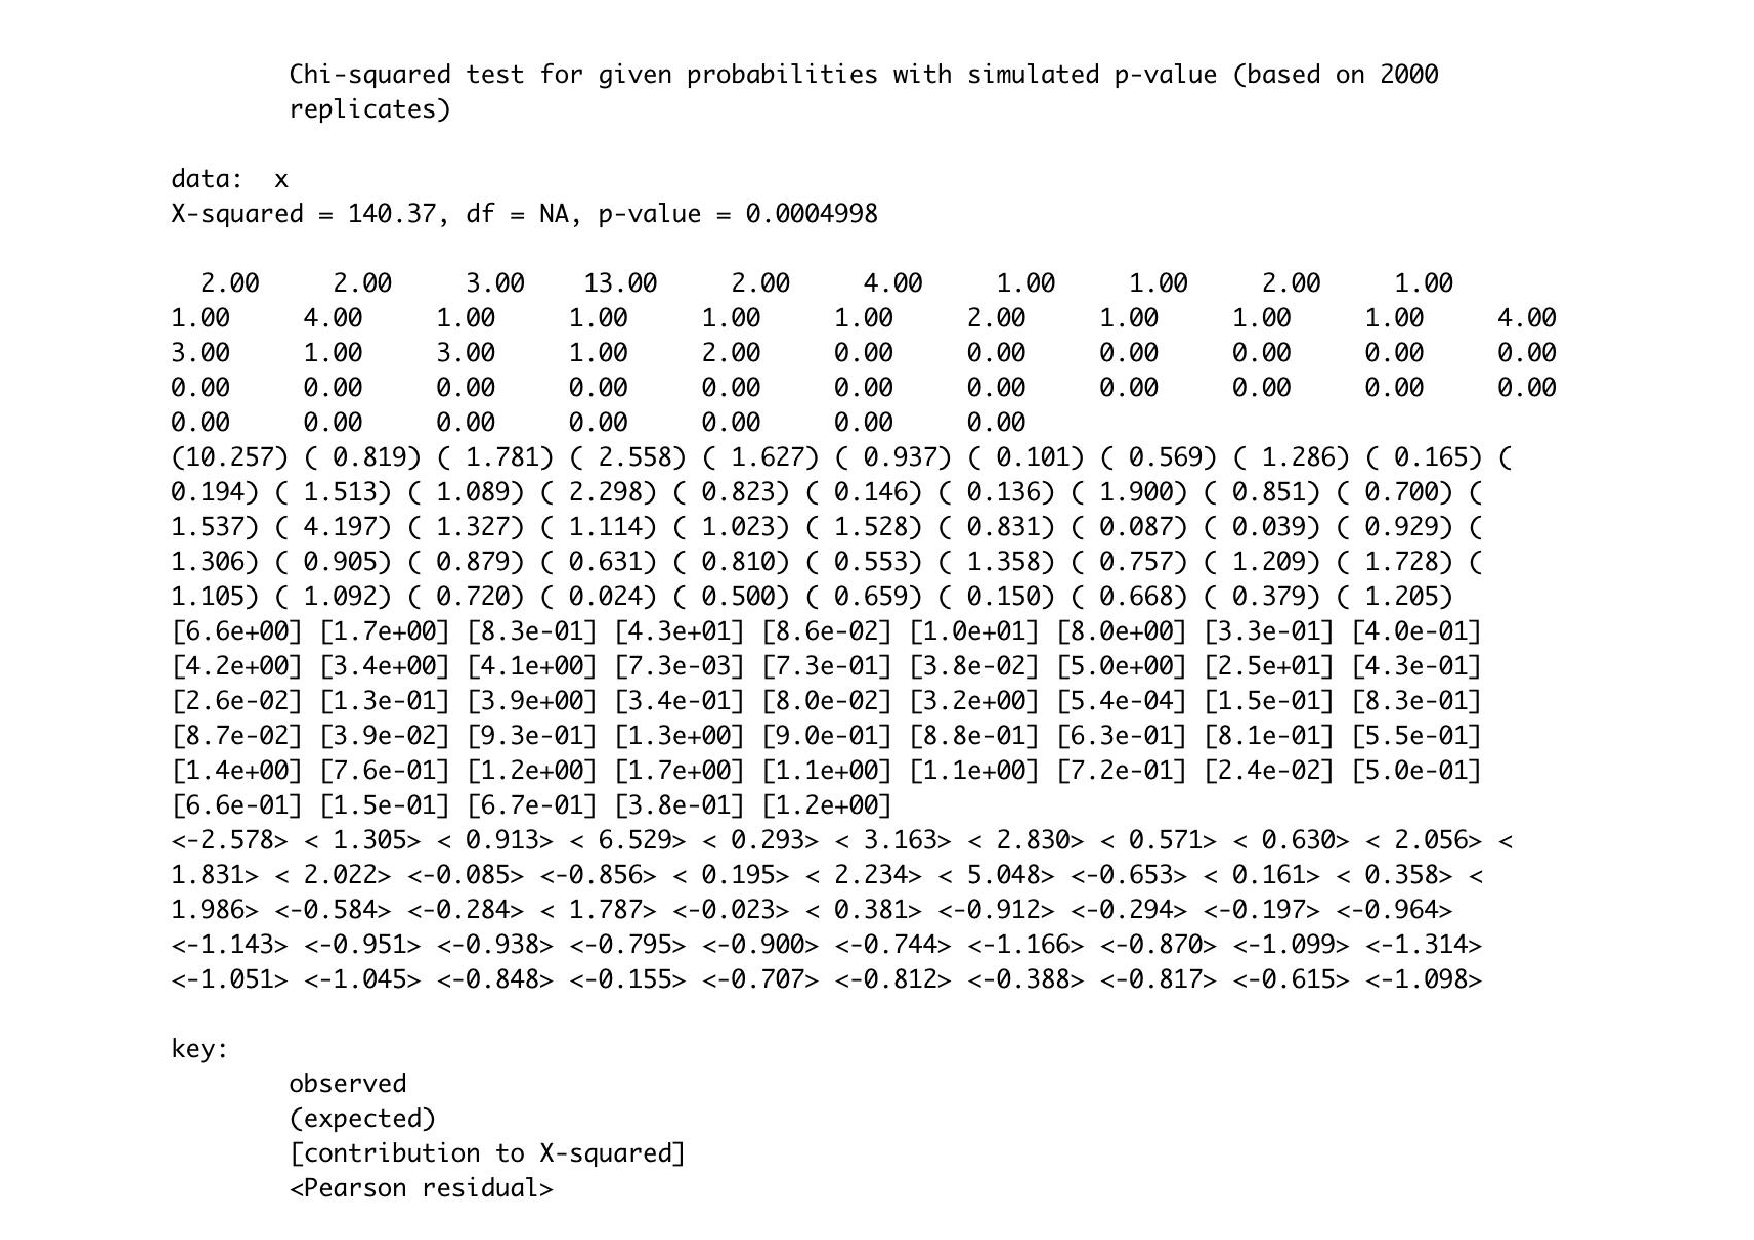
\includegraphics[width=10cm]{chi-state.pdf}
\end{figure}

From the Pearson residuals one can note that California has the most
positive residual thus, the observed frequency exceeds the expected
frequency. For a visual presentation, figure \emph{3} helps explain this
idea. The map on the left is what the map is expected to look like based
off of how large and small each state is. The map on the right is what
the map looks like when using the counts from the data set.

\begin{figure}
  \caption{Expected Frequency based on Square Mileage vs Observed Frequency}
    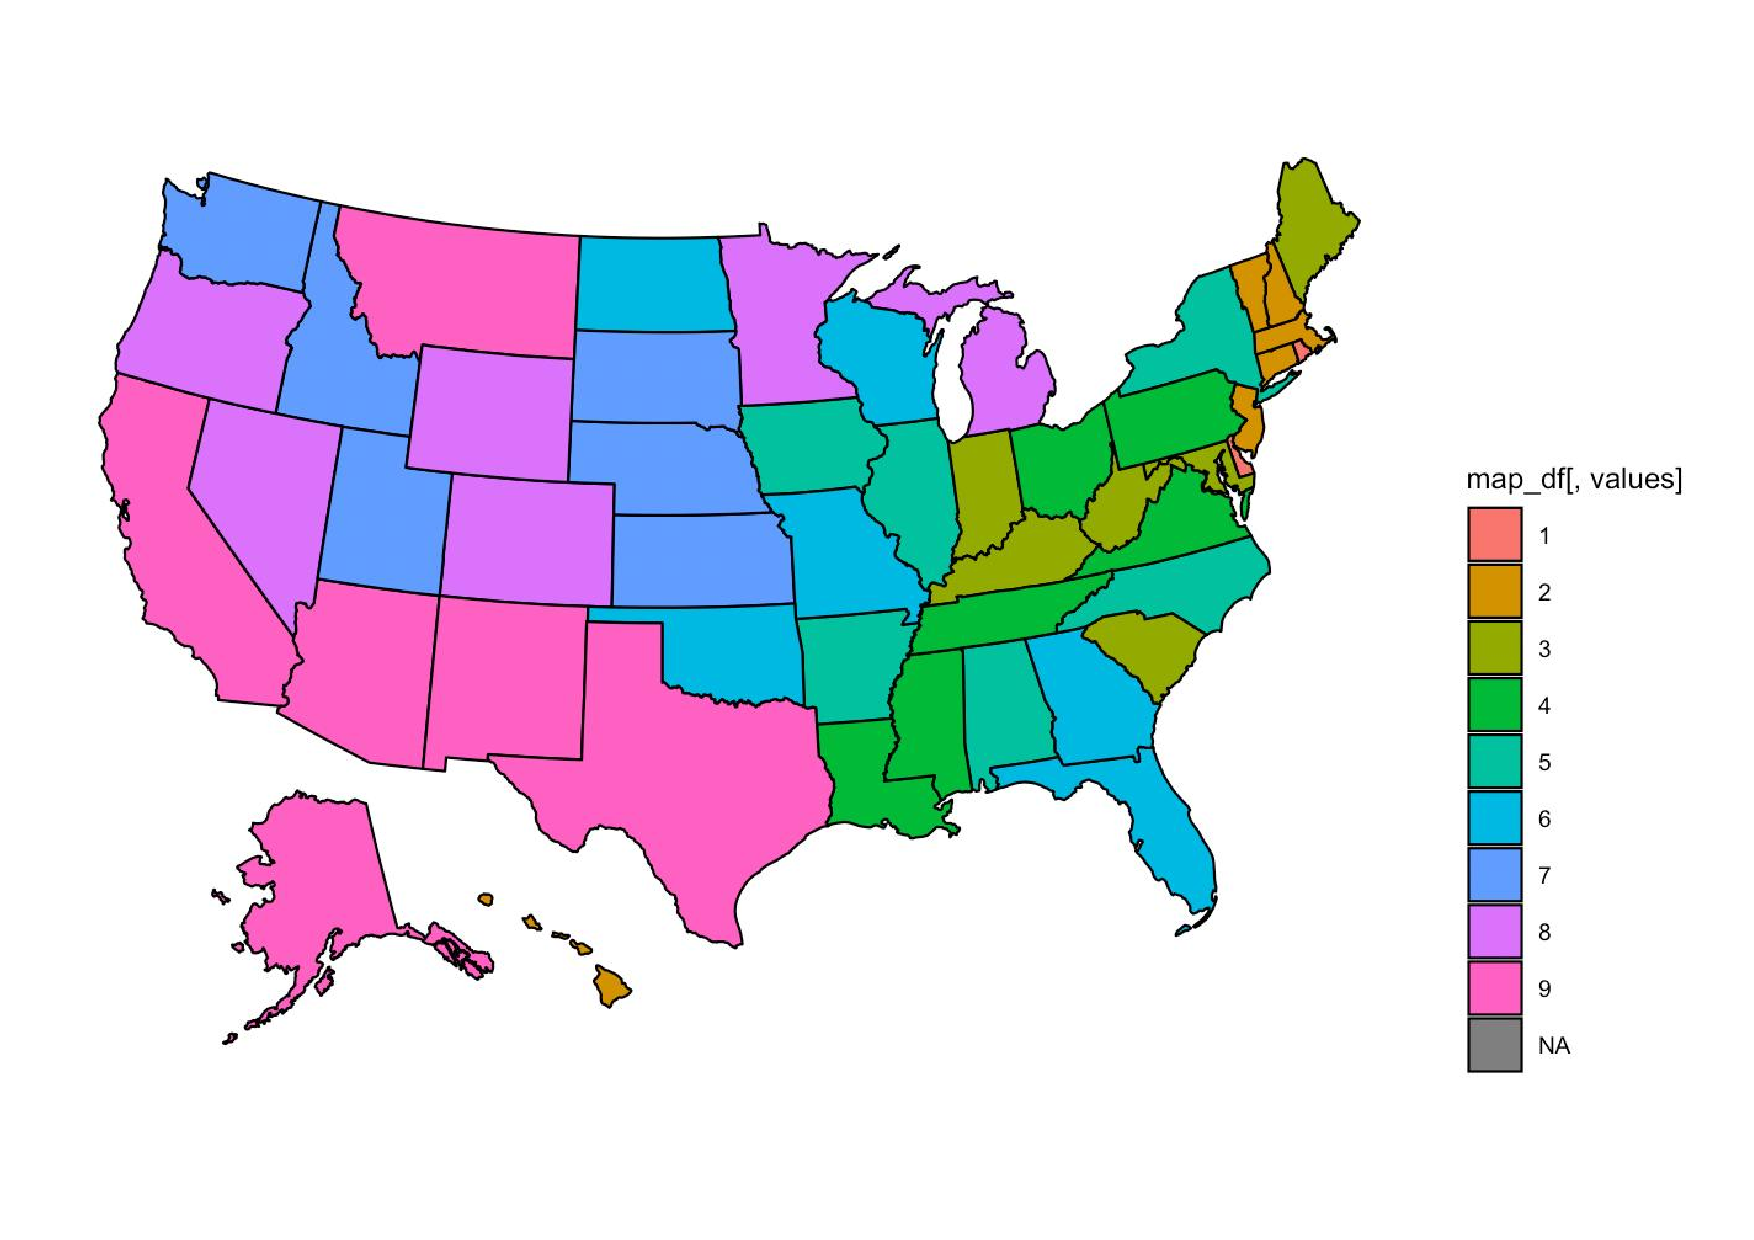
\includegraphics[width=7cm]{maps.pdf}
    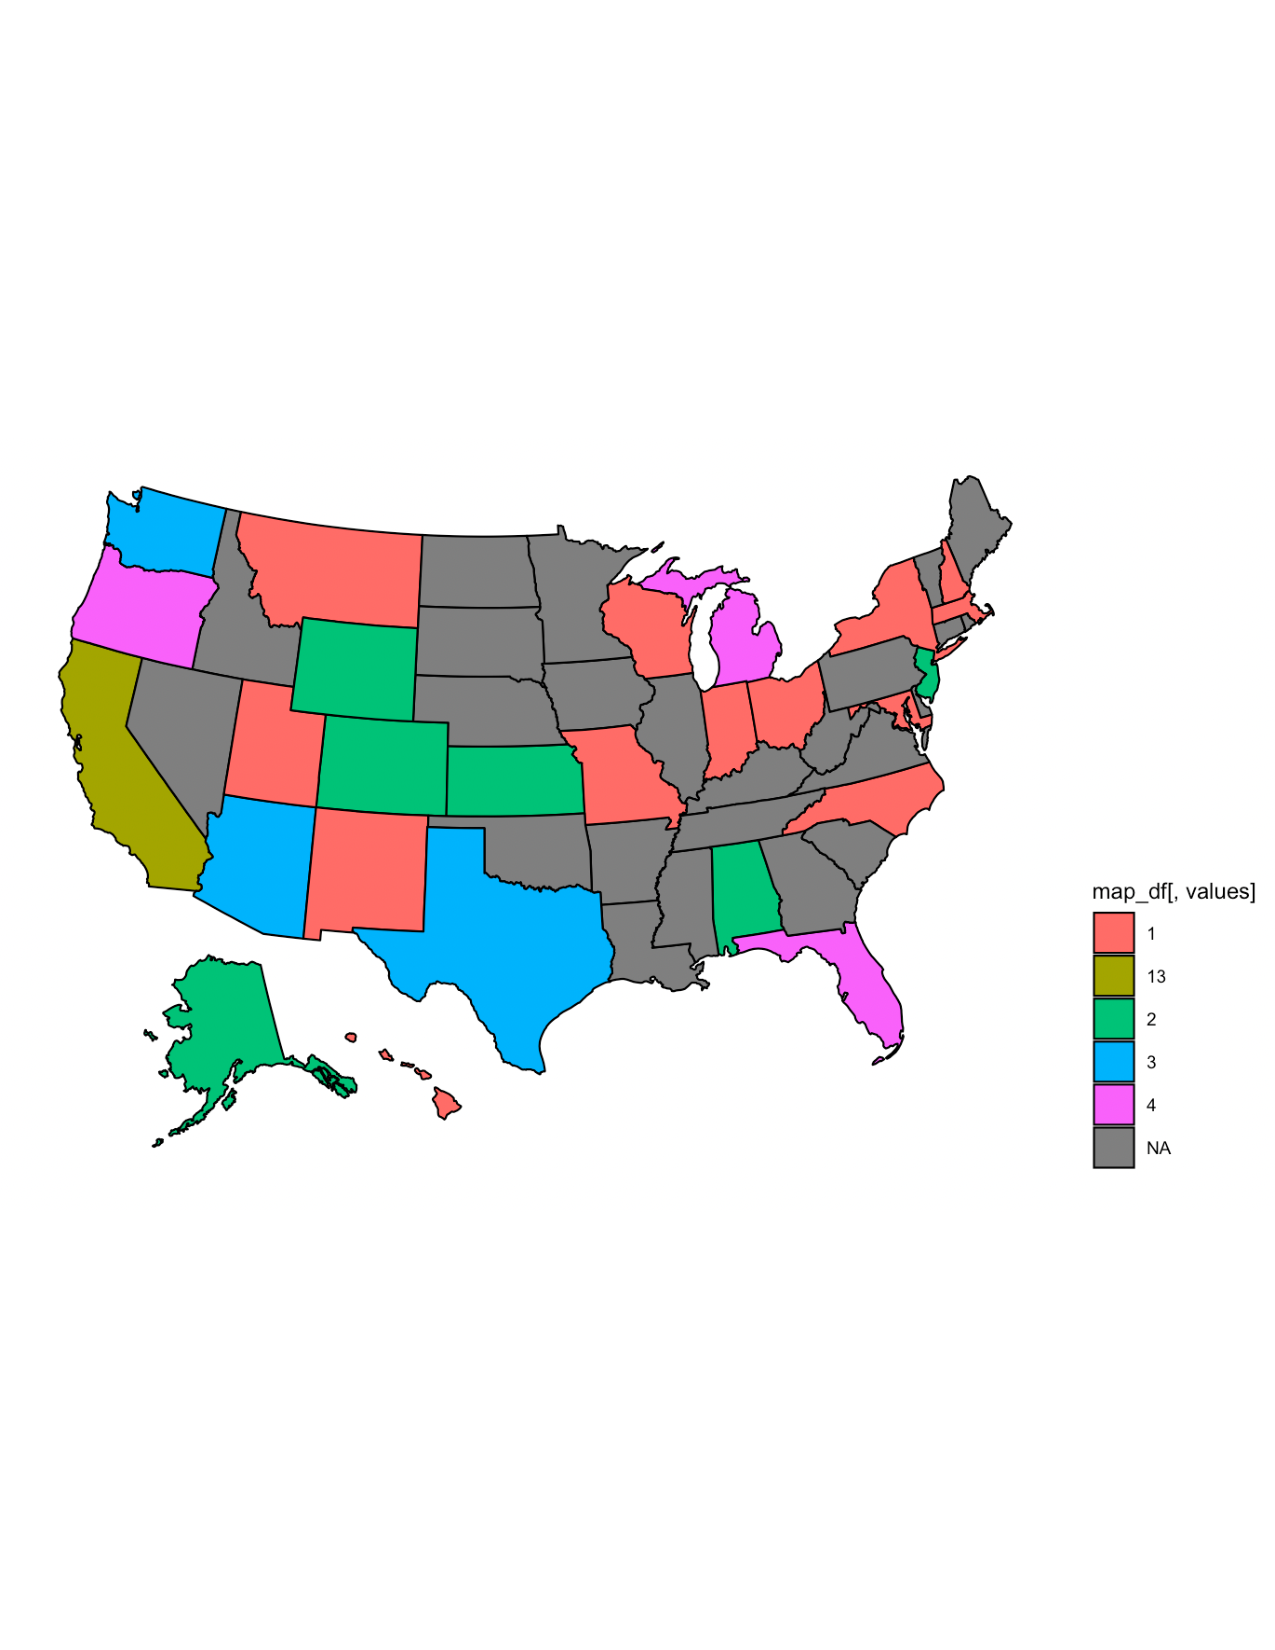
\includegraphics[width=7cm]{observed-map.pdf}
\end{figure}

California is a large state and the majority of the published articles
had work done in California. However, all the other states do not meet
the assumption. The gray states represent the sates that were never
counted in the data set. From the maps, one can conclude that the
probability of each state being represented in a journal entry is not
the same as the states square mileage. In other words, just because a
state is bigger does not mean there are more published articles from
that particular state.

\hypertarget{e.-ecosystem}{%
\subsection{e. Ecosystem}\label{e.-ecosystem}}

The ecosystem variable noted how many of the published articles used a
particular ecosystem. Ecosystems were broken down into 3 categories,
Marine, Terrestrial, and Freshwater. When looking at ecosystems, the
idea was to see if one ecosystem was counted more than a different
ecosystem. The following contingency table counts the number of times an
ecosystem was represented in the data set.

\begin{figure}
  \caption{Contingency Table}
    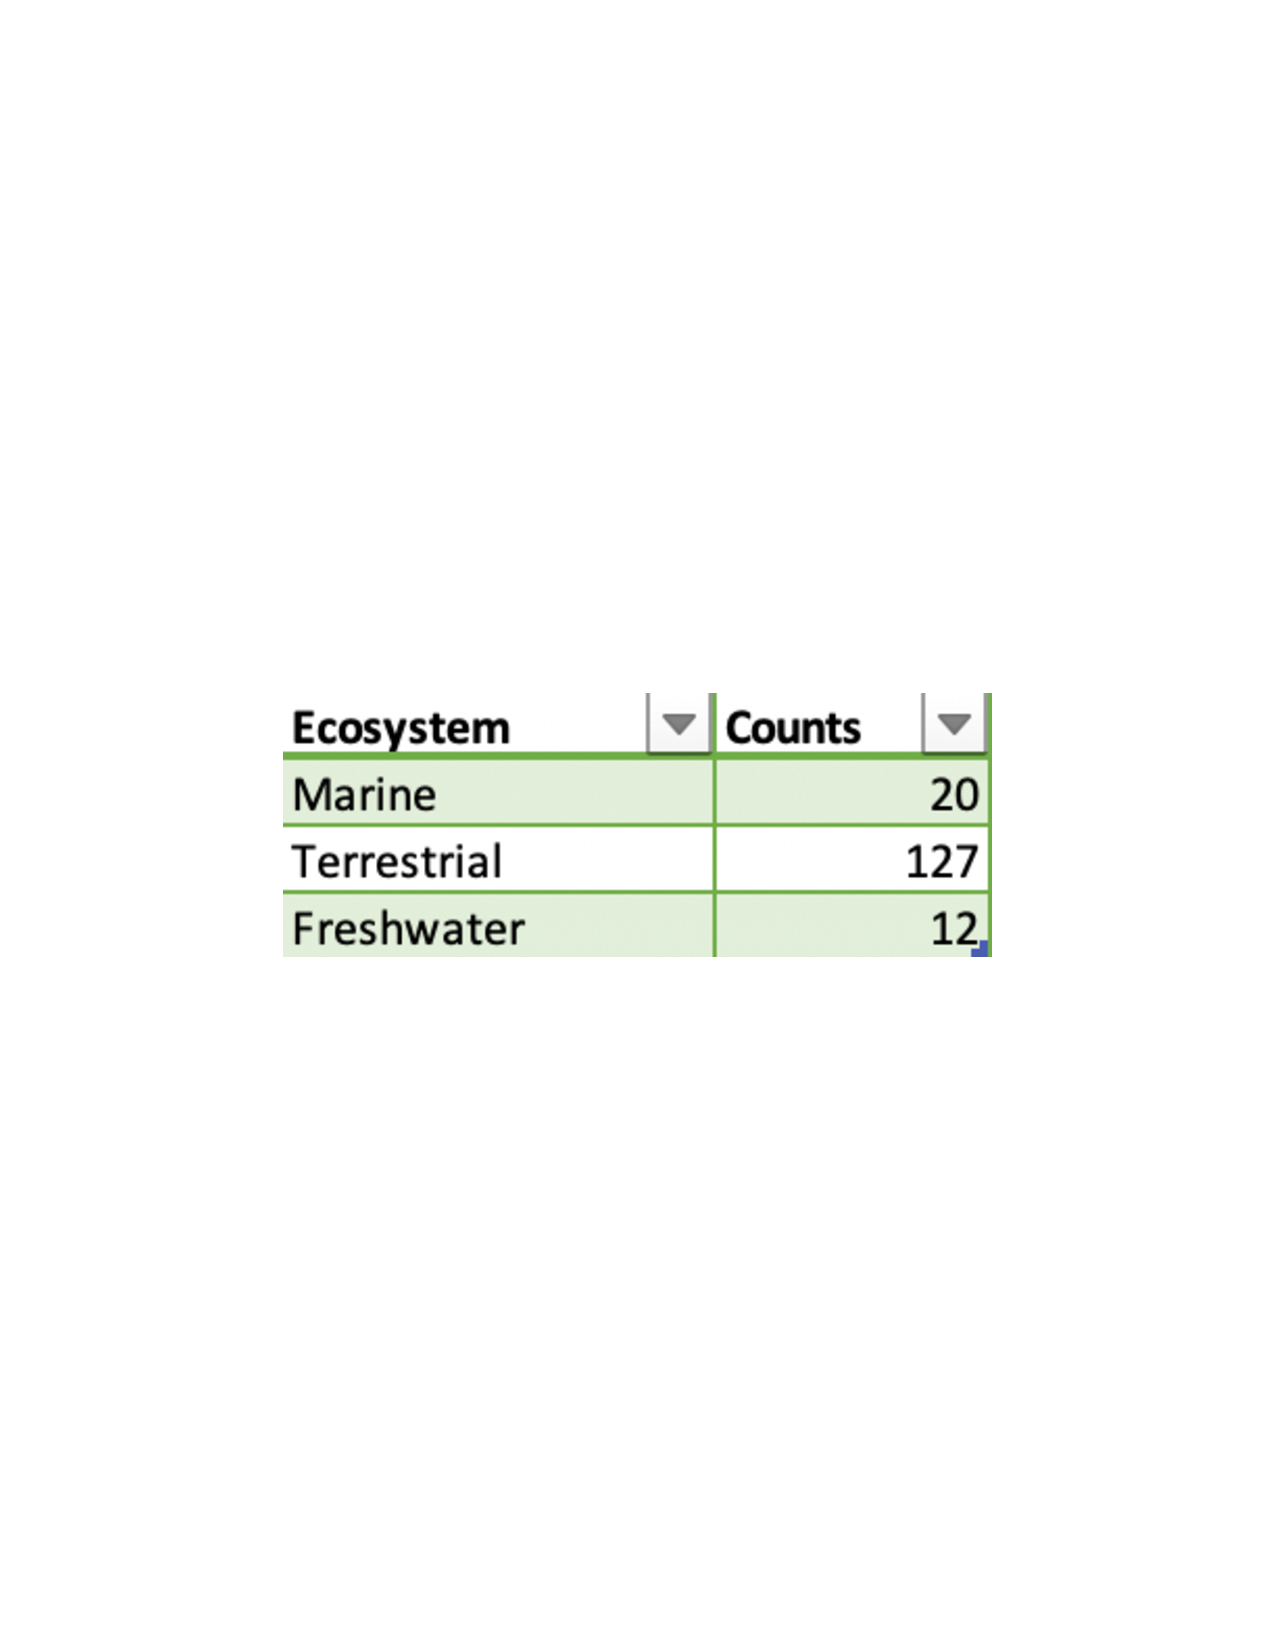
\includegraphics[width=13cm]{ct-eco.pdf}
\end{figure}

From the table above, one can tell that most of the published articles
have a terrestrial ecosystem. If there is an assumption that the
probability of each ecosystem being represented in a journal entry is
the same, then there should be the same number of counts for each
ecosystem. Below, is the Chi-Square test that test if this statement is
true.

\begin{figure}
  \caption{Chi-Square Test: Ecosystem}
    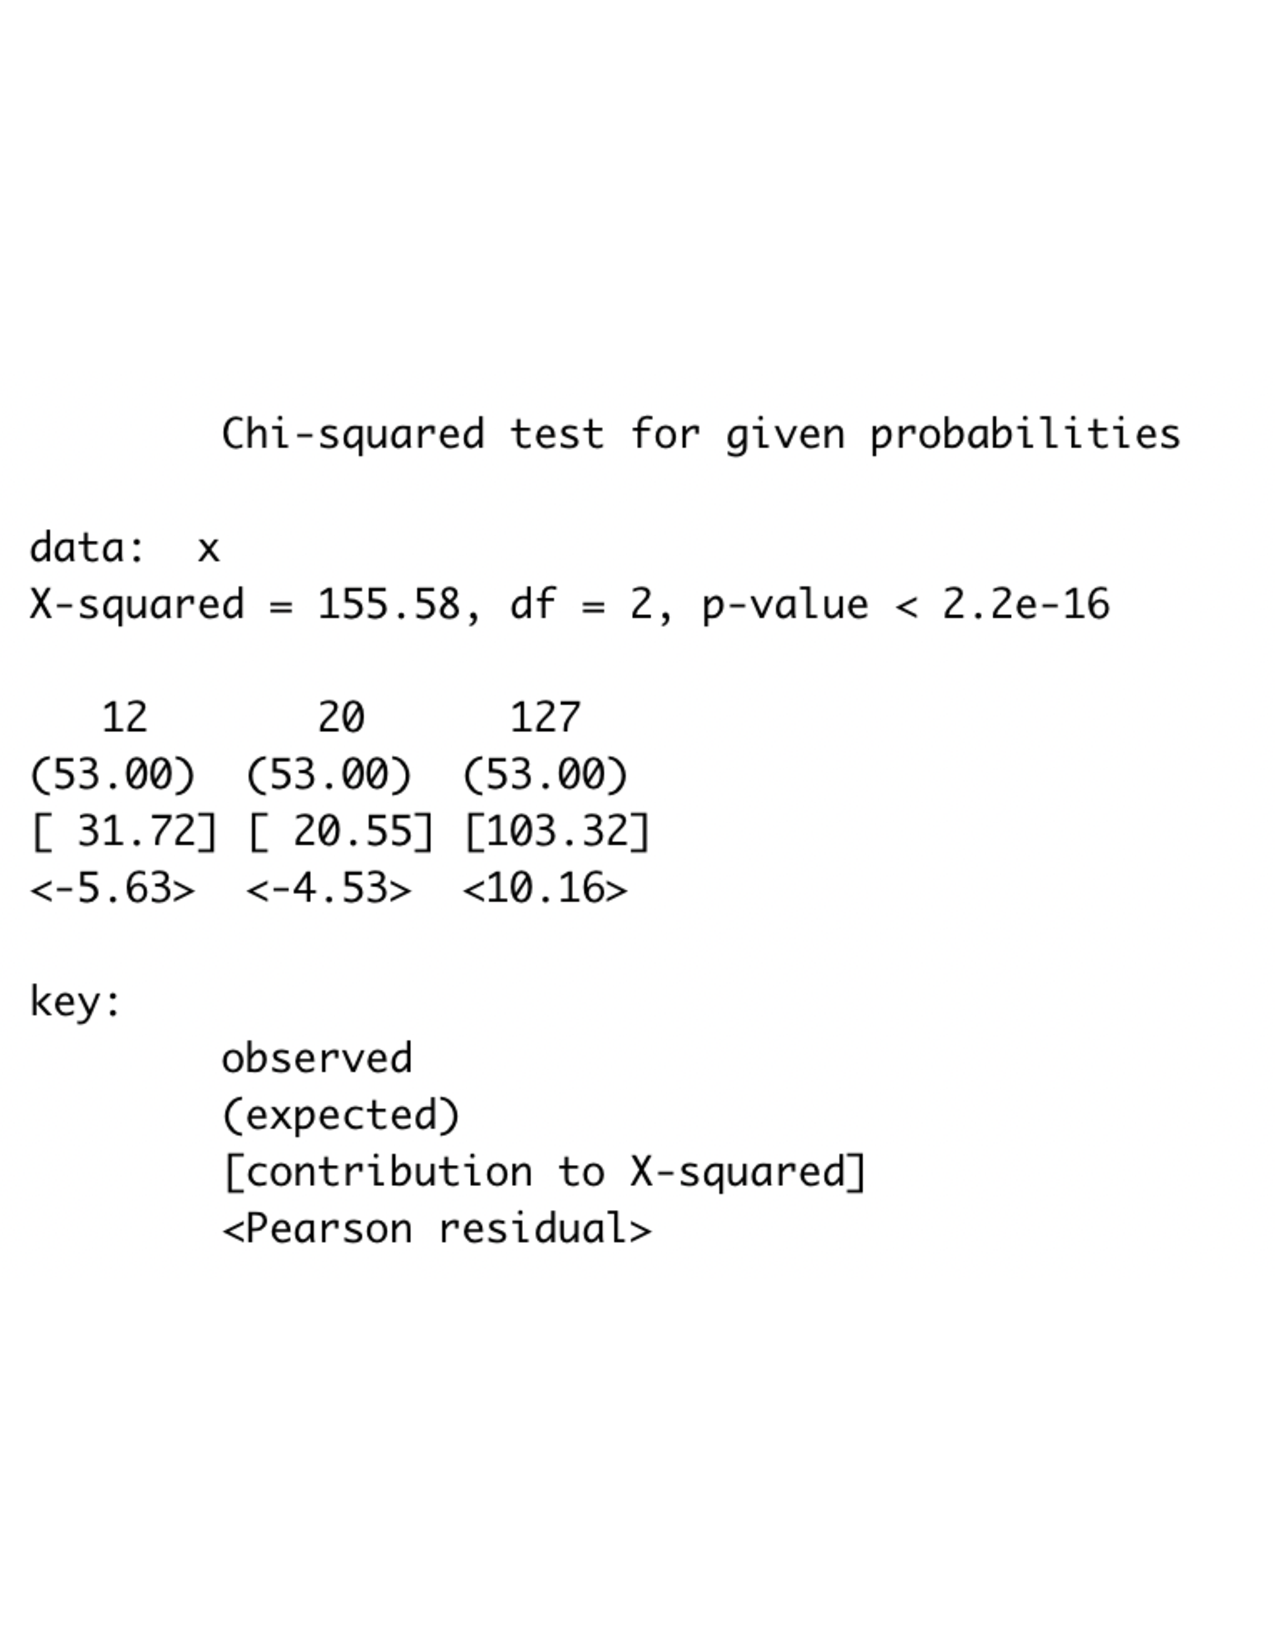
\includegraphics[width=10cm]{chi-eco-1.pdf}
\end{figure}

From the Pearson residuals one can note that terrestrial has the most
positive residual thus, the observed frequency exceeds the expected
frequency. Additionally,freshwater has the most negative residual thus,
the observed frequency does not meet the expected frequency. For a
visual presentation, figure \emph{3} helps explain this idea. The pie
chart on the left shows what the pie chart should look like if every
ecosystem had an equal chance of being represented in a published
article. While the pie chart on the right is what the pie chart looks
like when using the counts from the data set.

\begin{figure}
  \caption{Expected Frequency vs Observed Frequency}
    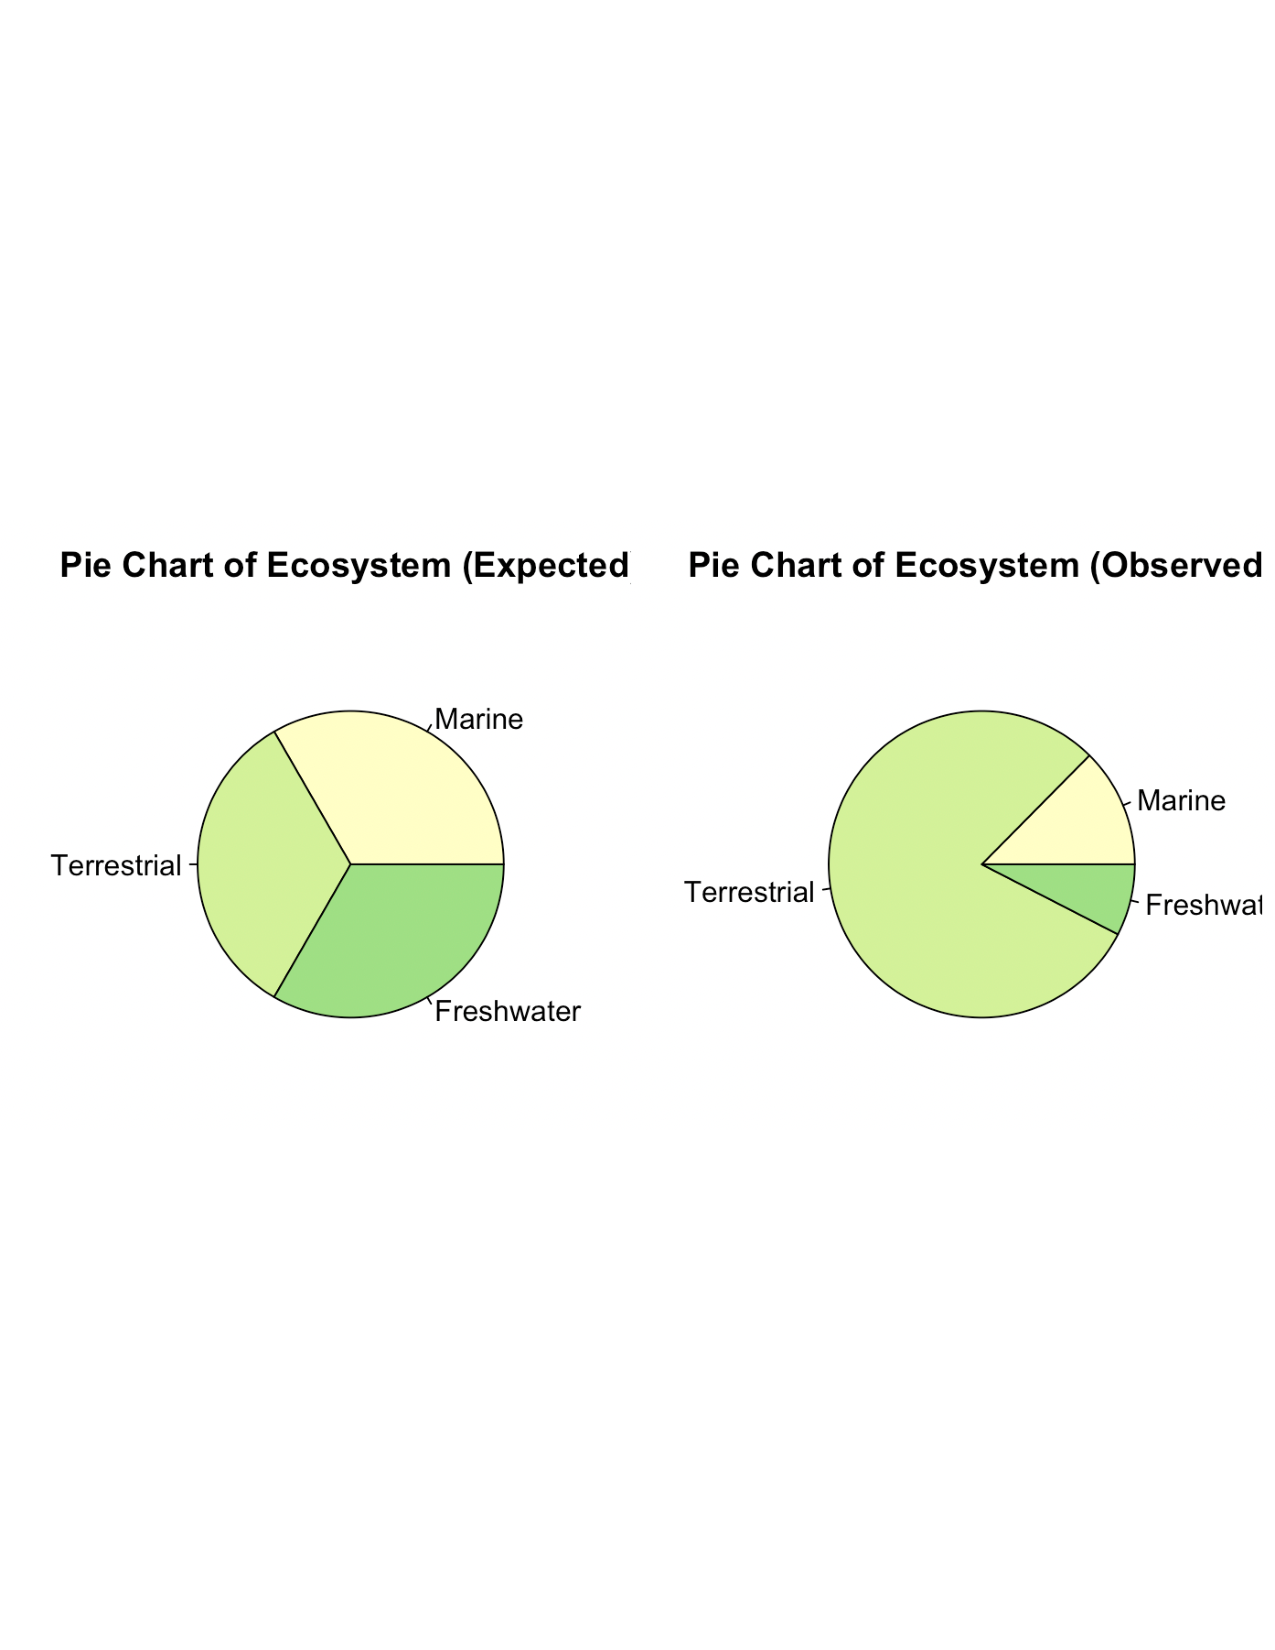
\includegraphics[width=10cm]{pie-eco-1.pdf}
\end{figure}

If the ecosystems had a equal chance of being represented in these
published articles these pie charts would look similar. However this is
not the case and it is obvious that terrestrial takes up the majority of
the pie chart.

If there is an assumption that the probability of each ecosystem being
represented in a journal entry is the same as each ecosystem's square
mileage then the larger ecosystem's would have more published articles
than the smaller ecosystems. Below, is the Chi-Square test that test if
this statement is true.

\begin{figure}
  \caption{Chi-Square Test: Ecosystem}
    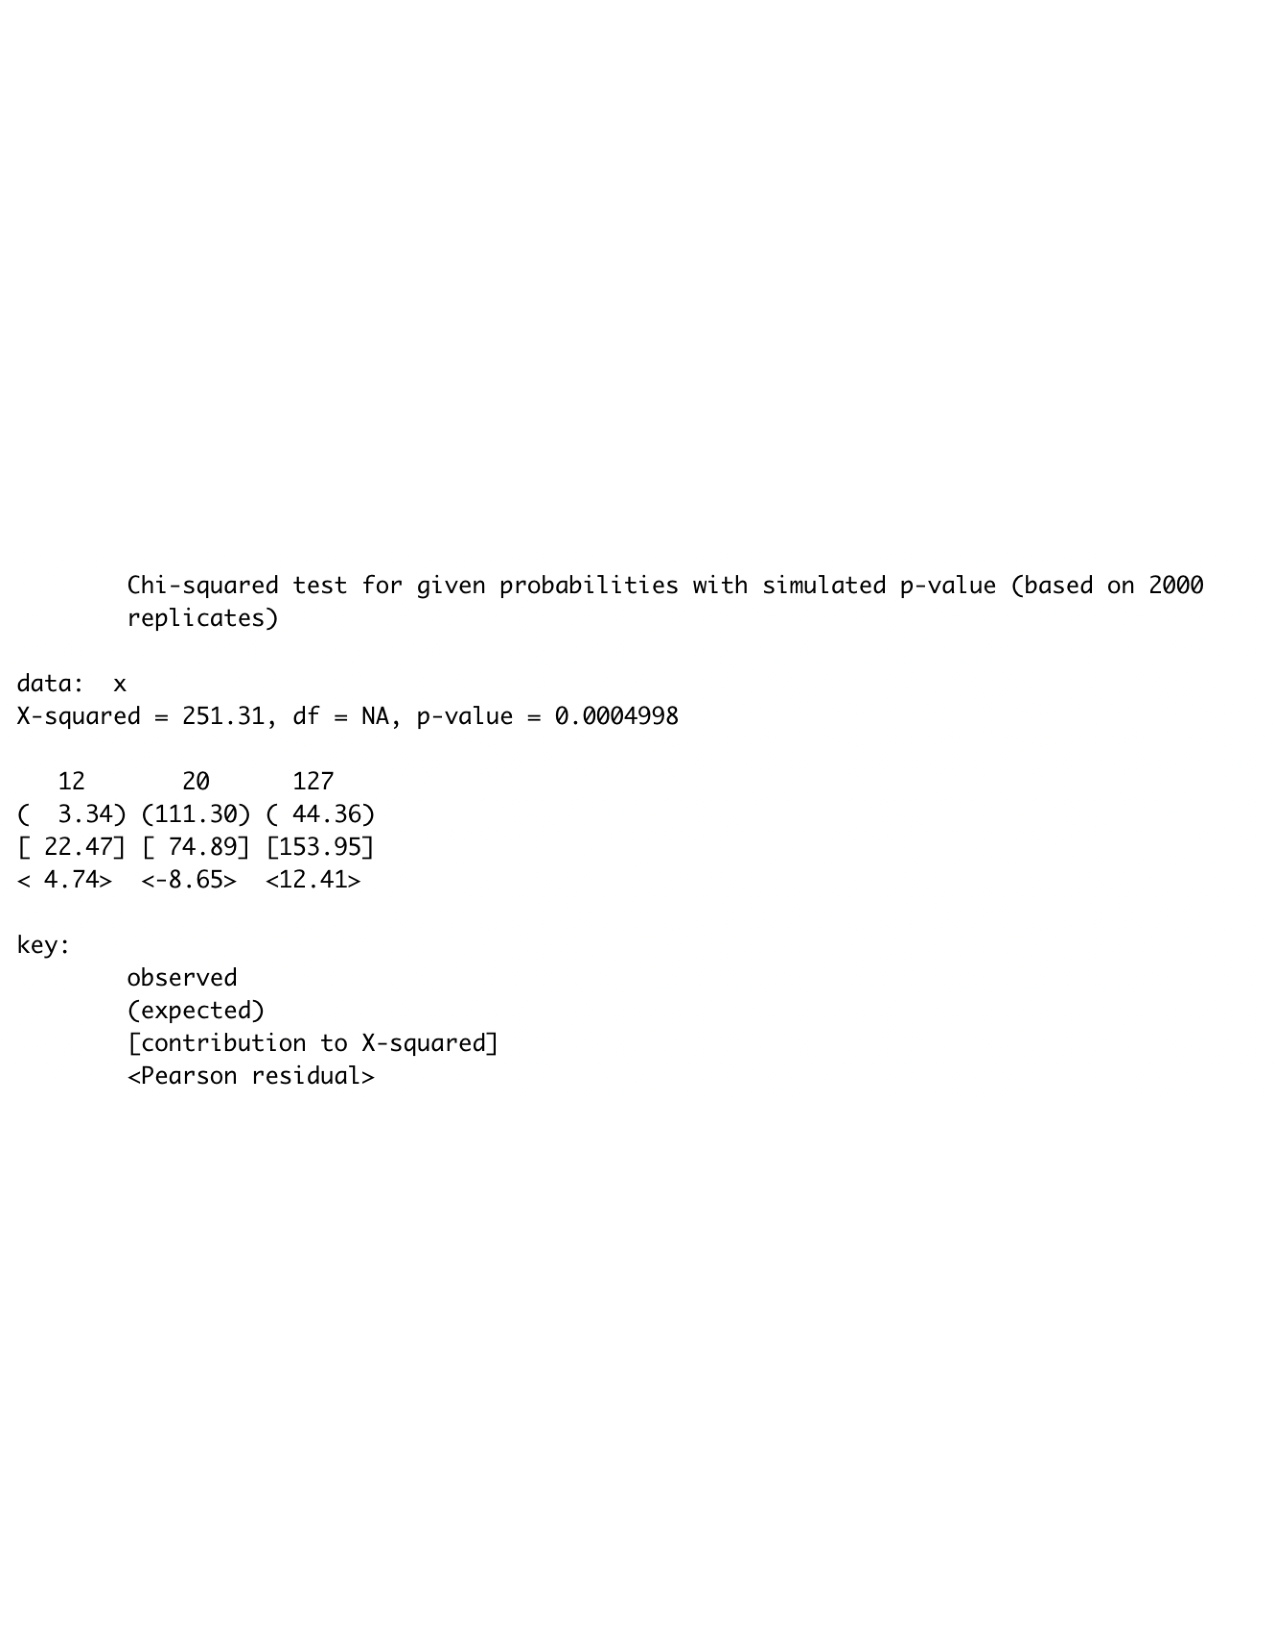
\includegraphics[width=10cm]{chi-eco-2.pdf}
\end{figure}

Terrestrial has the most positive residual and marine has the most
negative residual. Figure \emph{3} shows what the expected counts should
look like and what the observed counts were.

\begin{figure}
  \caption{Expected Frequency based on Square Mileage vs Observed Frequency}
    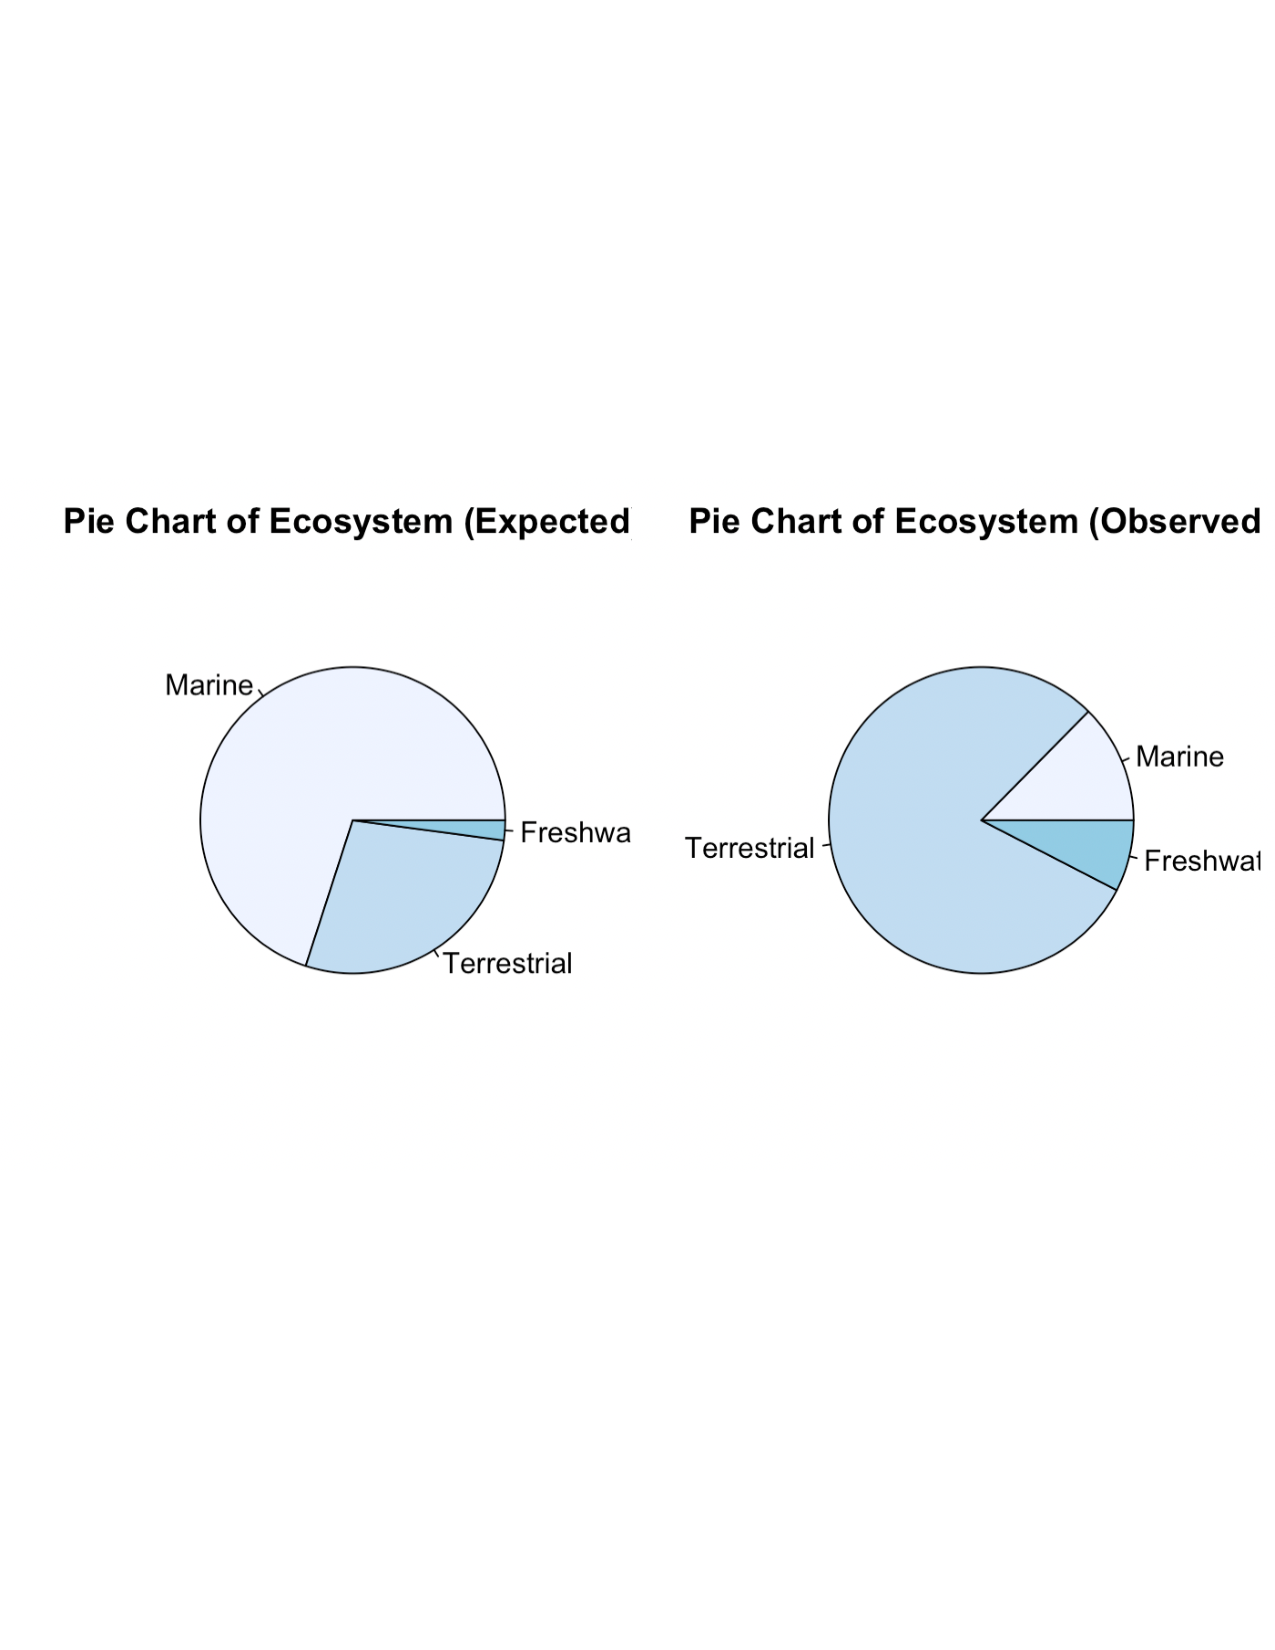
\includegraphics[width=10cm]{pie-eco-2.pdf}
\end{figure}

These bar charts do not match up thus, we cannot conclude that the
probability of each ecosystem being represented in a journal entry is
the same as each ecosystem's square mileage.

\hypertarget{discussion}{%
\section{Discussion}\label{discussion}}

Due to the data not being random and there only being qualitative
variables, there was not much statistical analysis to be done. For the
next time the study is done, we have come up with two different ways to
approach the study. If the research question was: Do publishing
companies publish more articles with work done in their region, in
comparison to work done outside of their region? The goal of using this
question is to eliminate the need for data on journal articles that were
not published. The study would focus on articles from different
publishing companies, but all from the same year. The regions from which
they published the most would be analyzed for any kind of bias. This
would be an observational study looking at the counts of journal
articles from each region.

Another approach would be to consider published articles that have
significant results. The research question is: Is there a greater
percentage of published articles that have a statistically significant
p-value (p \textless{} 0.05) in comparison to those who do not? The goal
of using this question would also be to eliminate the need for data on
journal articles that were not published, due to the population being
all published articles on ecology. This would be an observational study,
that would be conducted by looking at different publishing companies
from the same year and calculating the proportion of published articles
that had a p-value less than 0.05. This would be the test statistic used
to determine if there is any statistically significant difference in the
proportion of published articles with significant p-values.

Although both of these approaches fix the need for unattainable data,
they still do not fix meeting the randomness assumption. In order to fix
this, the data collectors can look for articles on a database, with the
criteria of the year they are looking for, the subject they want to look
into, and any other specifics they would like. After getting the results
of the search, they could use a random number generator to select which
articles they will use for their study. This will correct the issue of
the data not being randomly selected.

\end{document}
